%add something here
\documentclass[preprint]{sigplanconf}

\usepackage{times}
\usepackage{amsmath}
\usepackage{diagbox}
\usepackage{graphicx}
\usepackage{graphics}
\usepackage{epsfig}
\usepackage{epstopdf}
\usepackage{latexsym}
\usepackage{amsfonts}
\usepackage{amssymb}
\usepackage{paralist}
\usepackage{xspace}
\usepackage{mathrsfs}
\usepackage{amssymb}
\usepackage{color}
\usepackage{algorithm}
\usepackage{algorithmic}
\usepackage{listings}
\usepackage{multirow}
\usepackage{booktabs}
\usepackage{tabularx}
\usepackage{subfig}
\usepackage{caption}
\usepackage{url}
\usepackage{courier}
\usepackage{balance}
\usepackage{hyperref}

\usepackage{xcolor}
\hypersetup{
    colorlinks,
    linkcolor={red!50!black},
    citecolor={blue!50!black},
    urlcolor={blue!80!black}
}

\lstset{basicstyle=\footnotesize\ttfamily,breaklines=true}
\lstset{numbers=left}
\graphicspath{{figure/}}

%
% import the customized commands
%
\newcommand{\knote}[1]
{{$\langle${Kun: \textbf{#1}}$\rangle$}}
\newcommand{\kfnote}[1] {\footnote{\textcolor{red}{Kun: \it{#1}}}}
\newcommand{\todo}[1] {\textcolor{red}{To do: \it{#1}}}
\newcommand{\remove}[1] {{\textcolor{red}{\sout{#1}}}}
\newcommand{\add}[1] {{\textcolor{red}{\underline{#1}}}}
\newcommand{\egg}[1] {}
\newcommand{\separate}[1] {\textbf{\center ======  #1  ====== }}
\newcommand{\smalltitle}[1] {\vspace{6pt} \noindent \textbf{#1}}

\def\ie{\textit{i.e.}\xspace}
\def\etal{\textit{et al.}\xspace}
\def\etc{\textit{etc.}\xspace}
\def\eg{\textit{e.g.}\xspace}
\def\st{\xspace\textbf{s.t.}\xspace}
\def\whp{{\emph{w.h.p}}}
\def\cname{FICA \xspace}
\def\802{IEEE 802.11\xspace}
\def\arrow{$\rightarrow$}
\def\mrts{\textit{M-RTS}\xspace}
\def\mrtss{\textit{M-RTSes}\xspace}
\def\mcts{\textit{M-CTS}\xspace}
\def\mctss{\textit{M-CTSes}\xspace}
\def\approx{$\sim$}

\def\receivers{\textbf Q}
\def\capacity{{ \textbf{c}}}
\def\upperBound{{\mathcal D}}
\def\schedule{{\mathcal S}}
\def\throughput{{\cal T}}
\def\period{{\textbf Z}}

\newtheorem{theorem}{Theorem}
\newtheorem{axiom}[theorem]{Axiom}
\newtheorem{corollary}[theorem]{Corollary}
\newtheorem{definition}{Definition}
\newtheorem{lemma}[theorem]{Lemma}
\newtheorem{remark}[theorem]{Remark}

\newcommand{\prob}[1]{{\textbf{Pr}\left(#1\right)}}
\newcommand{\mcell}[2]{ \parbox[h]{#1}{ \vspace{0.5mm} #2 \vspace{0.5mm}}}

%\renewcommand\scriptsize{\@setfontsize\scriptsize\@viipt{9\p@}}
%\def\appsize{\@setsize\scriptsize{9\p@}\viipt\@viipt}

\lstdefinestyle{numbers} {numbers=left, stepnumber=1,
numberstyle=\tiny, xleftmargin=10pt, numbersep=5pt}
\lstset{language=C++}


\begin{document}
% only foreign words should be italicized
%\newcommand{\eg}{\textit{e.g.}}
%\newcommand{\ie}{\textit{i.e.}}
%\newcommand{\etal}{\textit{et al.}}
%\newcommand{\etc}{\textit{etc.}}
%\newcommand{\adhoc}{\textit{ad hoc}}

% general
\newcommand{\XXX}{{\bf XXX}}
\newcommand{\sref}[1]{\S\ref{#1}}
\newcommand{\oursys}{{KV-Direct}}
\newcommand{\ournic}{{programmable NIC}}
%\newcommand{\ourmodel}{{MEGA}}

% axes
\newcommand{\xaxis}{$x$-axis}
\newcommand{\yaxis}{$y$-axis}

% units
\newcommand{\KB}{~KB}
\newcommand{\MB}{~MB}
\newcommand{\GB}{~GB}
\newcommand{\MBs}{~MB/s}
\newcommand{\mus}{$\mu s$}
\newcommand{\ms}{$ms$}

\special{papersize=8.5in,11in}
\setlength{\pdfpageheight}{\paperheight}
\setlength{\pdfpagewidth}{\paperwidth}

%\titlebanner{banner above paper title}        % These are ignored unless
%\preprintfooter{short description of paper}   % 'preprint' option specified.

\title{KV-Direct: High-Performance In-Memory Key-Value Store with Programmable NIC \vspace{-0.1in}}

\authorinfo{Paper \#87 \vspace{-2in}}
           {}
           {}

\def\name{KV-Direct}
\def\fullname{Remote Direct Key-Value Access}
\def\sysname{}

\newcommand{\authornote}[1]{\raisebox{0.8ex}{$#1$}}
\maketitle

\newcommand{\specialcell}[2][c]{%
  \begin{tabular}[#1]{@{}c@{}}#2\end{tabular}}


\begin{abstract}

%This paper presents \oursys{}, a high-performance distributed in-memory key-value store (KVS). 
Performance of in-memory key-value store (KVS) continues to be of great importance as modern KVS goes beyond the traditional object-caching workload and becomes a key infrastructure to support distributed main-memory computation in data centers. 
%By leveraging FPGA based programmable network interface card (NIC) with several novel hardware and software designs innovations, \oursys{} aims to achieve performances that is close to the physical limit of the underlying hardware in terms of both throughput and latency.
Recent years have witnessed a rapid increase of network bandwidth in data centers, shifting the bottleneck of most KVS from the network to the CPU. RDMA capable NIC partly alleviates the problem, but the primitives provided by RDMA abstraction are rather limited. Meanwhile, programmable NICs become available in data centers, enabling in-network processing. In this paper, we present \oursys{}, a high performance KVS that leverages programmable NIC to extend RDMA primitives and enable remote direct key-value access to the main host memory. 

%In order to achieve performance that is close to the physical limits of the underlying hardware,
We develop several novel techniques to maximize the throughput and hide the latency of the PCIe connection between the NIC and the host memory, which becomes the new bottleneck. 
%To reduce the DMA request rounds through the PCIe bus, we adopt a novel FPGA friendly hash table and memory allocator design. To hide PCIe access latency and fully utilize the PCIe bandwidth, we design an out-of-order processing engine and a load-distribution component for host memory and on-board DRAM of our programmable NIC.
Combined, these mechanisms allow a single NIC \oursys{} to achieve up to 180 M key-value operations per second, equivalent to the throughput of tens of CPU cores. Compared with CPU based KVS implementation, \oursys{} improves power efficiency by 10\approx20x, while keeping tail latency below 10~$\mu$s. Moreover, \oursys{} can achieve near linear scalability with multiple NICs. With 8 programmable NIC cards in a server we achieve over one billion KV operations per second per server node, which is almost an order-of-magnitude improvement over existing systems, setting a new milestone for a general distributed key-value store.

%This paper presents KV-Direct, a high performance key-value store with programmable network interface card (NIC) which is deployed at scale in datacenters.
%KV-Direct extends RDMA primitives from memory operations to key-value operations, moves KV processing to the programmable NIC on server, thus enabling remote direct key-value access.
%In order to fully utilize PCIe bandwidth, we specialize hash table and slab memory allocator to minimize PCIe DMA requests for both GET and PUT operations.
%In order to hide PCIe latency, we design an out-of-order execution engine to issue independent KV operations while ensuring consistency.
%KV-Direct also leverages the DRAM on the NIC for caching and load balancing.
%A programmable NIC with KV-Direct can process up to 160M key-value operations per second, whose throughput is equivalent to 32 CPU cores, power efficiency is 16x higher than CPU, and tail latency is 10x lower than CPU.

%\oursys{} is an efficient in-memory key-value storage system based on \ournic{}.By offloading the KV operations to FPGA-based NIC, \oursys{} achieves 160\MBs{} key-value operations, whose throughput is equivalent to 32 CPU cores, power efficiency is 16x higher than CPU, and tail latency is 10x lower than CPU, up to 5\mus{}. 
%Besides, \oursys{} is in linear scale to multiple programmable NICs, achieving one billion KV op/s per-server, more than an order-of-magnitude improvement over existing systems, setting a new milestone for key-value storage system.

%Recent years we witness the trend of the end of processor frequency scaling and multi-core scaling, as well as the widely deployment of \ournic{} in datacenter, which offers the great opportunity for us to redesign the key-value system. 
%In \oursys{}, we extend the RDMA primitives to key-value operations with consistency guarantee while keeping its CPU-bypass semantics. 
%To optimize the new bottleneck in PCIe and reduce the DMA requests, we adopts a new FPGA friendly hash table and memory allocation design.
%Furthermore, to guarantee the consistency and leverage FPGA parallism, we design an hardware based out-of-order engine and a load-balancing component for on-board cached DRAM and host memory.
%Combined, these mechanisms allow KV-Direct to achieve high throughput and low latency for both GET and PUT key-value operations. 

\end{abstract}
\section{Introduction}
\label{sec:introduction}

%\subsection{outline}
%
%KV is an important infrastructure service
%
%Existing solution of key-value store in
%
%1. CPU-based
%
%2. RDMA-based
%
%recent trend of programmable NIC in datacenter
%
%we present KV-Direct... 
%
%highlight the high level insight (offload the simple and performance critical operation to programmable NIC) 
%
%and design goal and spotlight (not only match the state of art of RDMA-based solution in GET operation and significant improve the PUT operation to even comparable to CPU-based solution. Moreover, our solution is more power and cost effective. With more FPGA or the improvement of FPGA, we can beat all existing CPU/RDMA solution.)
%
%KV-Direct makes contributions in three main aspects:
%
%1. proposes a KV solution for programmable NIC to Direct Memory Access.
%
%2. extends RDMA primitives to Key-value operation with consistency guarantee while high performance. 
%
%3. makes critical PCIe traffic optimization in our novel FPGA-based NIC key-value service design.



%Key-value store (KVS) is an infrastructure service to store shared structured data in a distributed system.
%Traditionally, the performance of KVS is mostly constrained by the OS network stack.
%Recent research leverage two-sided RDMA to accelerate communication among clients and KVS servers.
%The next bottleneck is CPU. The KV operation throughput of a CPU core is constrained by its latency hiding efficiency and computation capacity.
%Another approach is to use one-sided RDMA to bypass remote CPU and move KV processing to clients, but it incurs high communication and synchronization overhead.
%\subsection{current version}



\begin{figure*}[t]
\centering
\subfloat[Software / two-sided RDMA.\label{fig:memaccess-a}]
{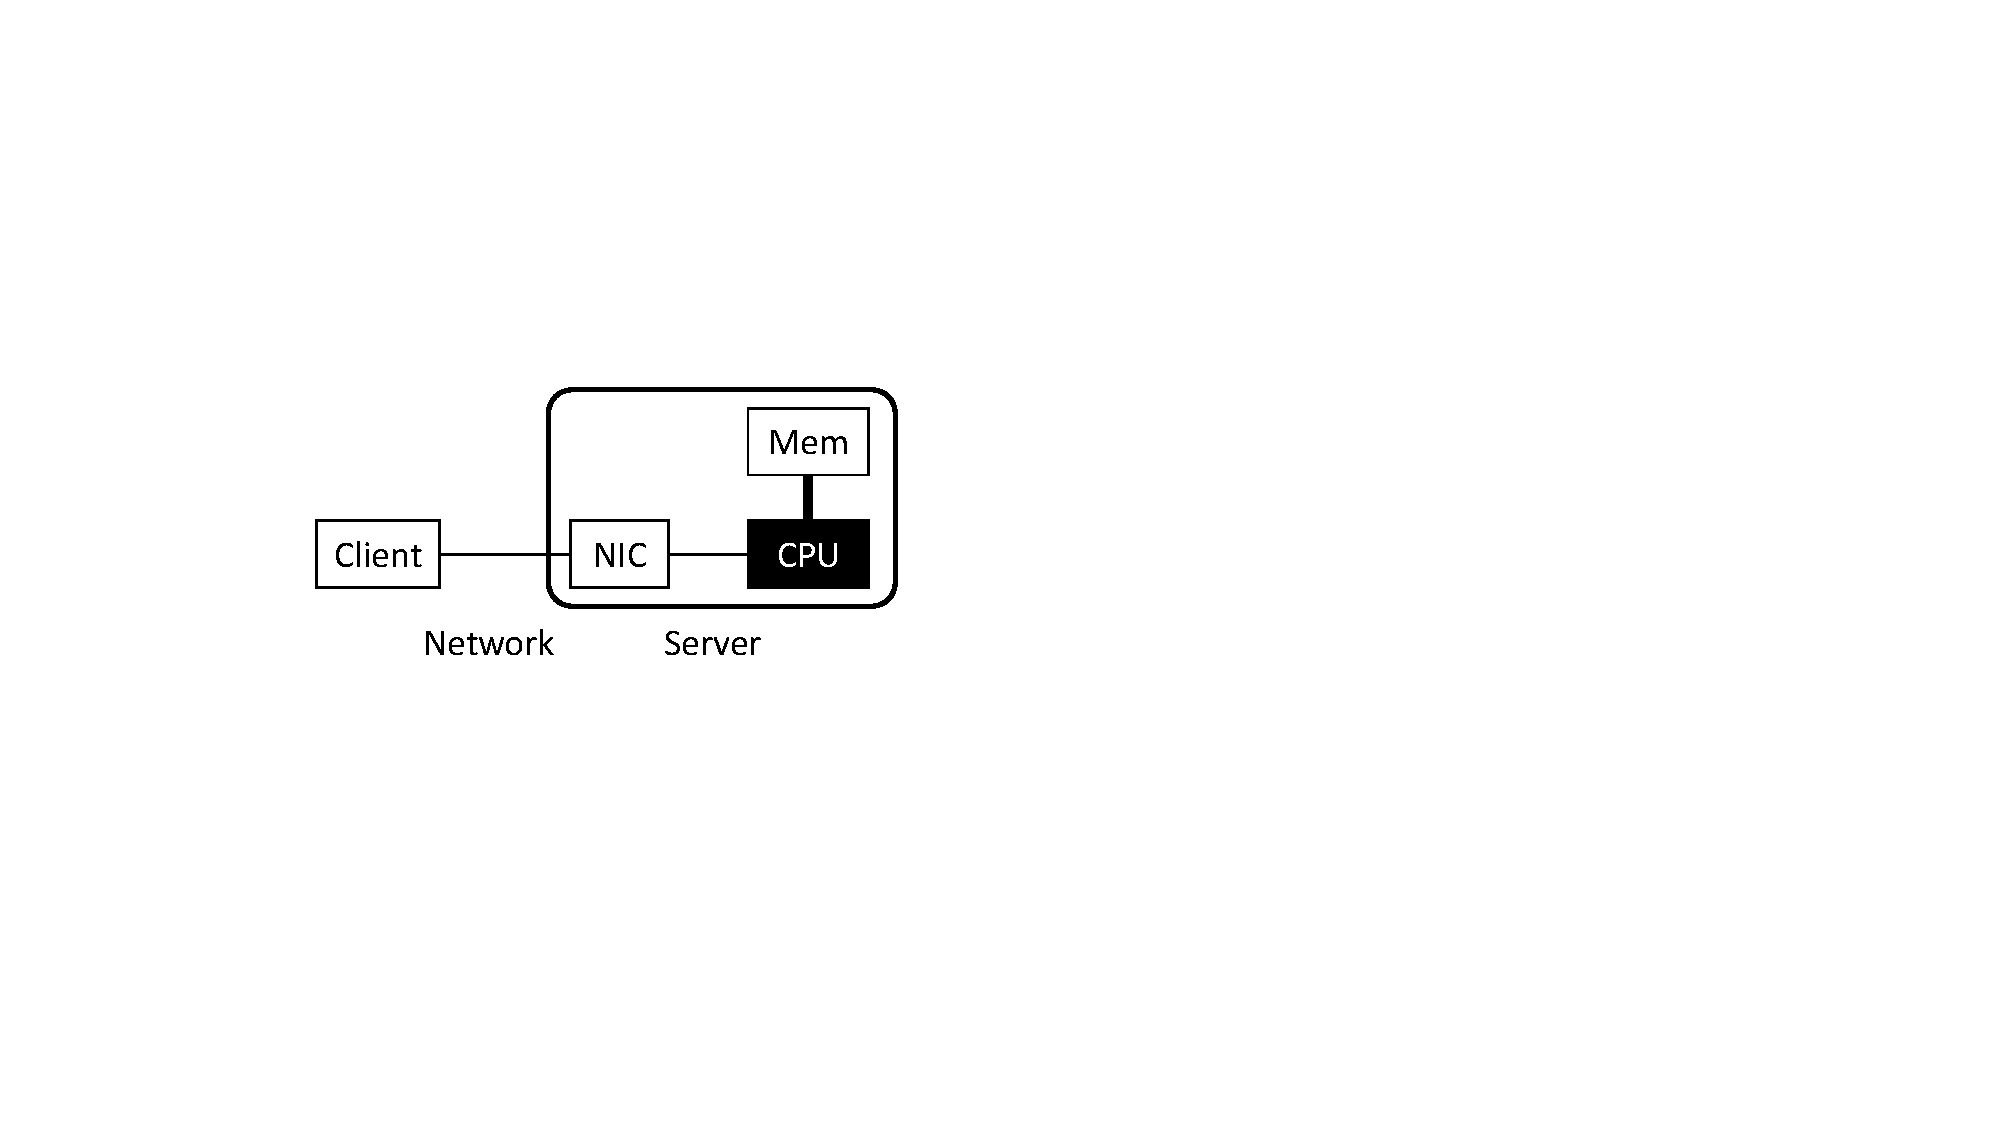
\includegraphics[width=.3\textwidth,page=1]{cropped_access.pdf}}
\subfloat[One-sided RDMA.\label{fig:memaccess-b}]
{\includegraphics[width=.3\textwidth,page=2]{cropped_access.pdf}}
\subfloat[KV-Direct.\label{fig:memaccess-c}]
{\includegraphics[width=.3\textwidth,page=3]{cropped_access.pdf}}
\caption{Design space of KVS data path and processing device. Line indicates data path. One KV operation (thin line) may require multiple address-based memory accesses (thick line). Black box indicates where KV processing takes place.}
\label{fig:memaccess}
\vspace{-10pt}
\end{figure*}

In-memory key-value store (KVS) is a key distributed system component in many data centers. KVS enables access to a shared key-value hash table among distributed clients. Historically, KVS such as Memcached~\cite{fitzpatrick2004distributed} gained popularity as an object caching system for web services. Large web service providers such as  Amazon~\cite{decandia2007dynamo} and Facebook~\cite{atikoglu2012workload, nishtala2013scaling}, have deployed distributed KVSs at scale. More recently, as main-memory based computing becomes a major trend in the data centers~\cite{ousterhout2010case,dragojevic2014farm}, KVS starts to go beyond caching and becomes an infrastructure to store shared data structure in a distributed system.
Many data structures can be expressed in a key-value hash table, \eg, data indexes in NoSQL databases~\cite{chang2008bigtable}, model parameters in machine learning~\cite{li2014scaling}, nodes and edges in graph computing~\cite{shao2013trinity, xiao17tux2} and sequencers in distributed synchronization~\cite{kalia2016design}. For most of these applications, the performance of the KVS is the key factor that directly determines the system efficiency. Due to its importance, over the years significant amount of research effort has been invested on improving KVS performance. 

Earlier key-value systems~\cite{decandia2007dynamo, fitzpatrick2004distributed, nishtala2013scaling} are built on top of traditional OS abstractions such as OS lock and TCP/IP stack. This puts considerable stress on the performance of the OS, especially the networking stack. The  bottleneck is exacerbated by the fact that physical network transport speed has seen huge improvements in the last decade due to heavy bandwidth demand from data center applications. 

More recently, as both the single core frequency scaling and multi-core architecture scaling are slowing down~\cite{sutter2005free,esmaeilzadeh2011dark}, a new research trend in distributed systems is to leverage Remote Direct Memory Access (RDMA) technology on NIC to reduce network processing cost. One line of research~\cite{kalia2014using, kalia2016design} uses two-sided RDMA to accelerate communication (Figure~\ref{fig:memaccess-a}). KVS built with this approach are bounded by CPU performance of the KVS servers. Another line of research uses one-sided RDMA to bypass remote CPU and shift KV processing workload to clients~\cite{dragojevic2014farm, mitchell2013using} (Figure~\ref{fig:memaccess-b}). This approach achieves better GET performance but degrades performance for PUT operations due to high communication and synchronization overhead. It is evident that the limited abstraction provided by RDMA is not a perfect fit for building efficient KVS. 

In the meantime, another trend is emerging in data center hardware evolution. More and more servers in data centers are now equipped with \ournic{}s~\cite{caulfield2016cloud, greenberg2015sdn,putnam2014reconfigurable}.
At the heart of a programmable NIC is a field-programmable gate array (FPGA) with an embedded NIC chip to connect to the network and a PCIe connector to attach to the server.
Programmable NIC is initially designed to enable network virtualization~\cite{vfp,li2016clicknp}.
However, many found that FPGA resources can be used to offload some workloads of CPU and significantly reduce CPU resource usage~\cite{ouyang14hotchips, MaZC17fpga, huang16socc, cong16dac}. Our work takes this general approach.

We present \oursys{}, a new in-memory key-value system that takes advantage of \ournic{} in data center.
\oursys{}, as its name implies, directly fetches data and applies updates in the host memory to serve KV requests, bypassing host CPU (Figure~\ref{fig:memaccess-c}).
%We leverage the insight of one-sided RDMA-based KV systems to bypass CPU, while offload the computation logic to FPGA-based NIC to ensure the consistency in server side, which results in the remarkable performance improvement through network traffic reduction and less synchronization overhead, furthermore, the client side becomes transparent to all KV operations.
\oursys{} extends the RDMA primitives from memory operations (READ and WRITE) to key-value operations (GET, PUT, DELETE and ATOMIC ops). Compared with one-sided RDMA based systems, \oursys{} deals with the consistency and synchronization issues at server-side, thus remove the computation load in client and reduce network traffic.
In addition, to support vector-based operations and reduce network traffic, \oursys{} also provides new vector primitives UPDATE, REDUCE, and FILTER, allowing users to define active messages~\cite{eicken1992active} and delegate certain computation to programmable NIC for efficiency.

Since the key-value operations are offloaded to the \ournic{}, we focus our design on optimizing the PCIe traffic between the NIC and host memory. \oursys{} adopts a series of optimizations to fully utilizing PCIe bandwidth and hide latency. Firstly, we design a new hash table and memory allocator to leverage parallelism available in FPGA and minimize the number of PCIe DMA requests. On average, \oursys{} achieves close to one PCIe DMA per READ operation and two PCIe DMAs per WRITE operation. Secondly, to guarantee consistency among dependent KV operations, \oursys{} includes an out-of-order execution engine to track operation dependencies while maximizing the throughput of independent requests. Thirdly, \oursys{} exploits on-board DRAM buffer available on \ournic{} by implementing a hardware-based load dispatcher and caching component in FPGA to fully utilize on-board DRAM bandwidth and capacity. 

%%\textbf{TODO:performance highlight}
%three key results:
%
A single NIC \oursys{} is able to achieve up to 180~M KV operations per second (Ops), equivalent to the throughput of 36 CPU cores~\cite{li2016full}. Compared with state-of-art CPU KVS implementations, \oursys{} reduces tail latency to as low as 10~\mus{} while achieving a 10\approx20x improvement on power efficiency. Moreover, \oursys{} can achieve near linear scalability with multiple NICs. With 8 \ournic{} cards in a server we achieve one billion KV operations per second per server node, which is more than an order of magnitude improvement over existing systems.

\oursys{} supports general atomic operations up to 180~Mops, equal to normal KV operation and significantly outperforms the number reported in state-of-art RDMA-based system: 2.24~Mops~\cite{kalia2014using}. The atomic operation agnostic performance is mainly a result of our out-of-order execution engine that can efficiently track the dependency among KV operations without explicitly stalling the pipeline.

%The rest of the paper is organized as follows. \S\ref{sec:background} shows the background, clarifies our design goals as well as challenges. \S\ref{sec:architecture} describes \oursys{} design. \S\ref{sec:implementation} presents the implementation details of \oursys{}. \S\ref{sec:evaluation} is the evaluation of \oursys{}. \S\ref{sec:extensions} talks about the further extensions. We discuss the related work in \S\ref{sec:related} and conclude in \S\ref{sec:conclusion}.

\section{Background}
\label{sec:background}


\egg{
\subsection{The Road to High Performance KVS}

Building a high performance KVS is a non-trivial exercise of optimizing various software and hardware components in a computer system. The rich literature on KVS performance optimizations can give us a glimpse of software and hardware evolution in recent years.
Early works on distributed in-memory KVS such as Memcached~\cite{fitzpatrick2004distributed} uses OS locks for multi-core synchronization and TCP/IP networking stack for communication. Since then, optimizations have been made on multiple fronts to remove bottlenecks in various parts of the system.


\subsubsection{Synchronization cost}
\label{sec:CoreSynchronizationCost}
Synchronization is needed in multi-threaded KVS implementation since multiple clients might access the same keys concurrently. For example, when two clients make atomic increments to a single key, the value needs to reflect both increments.

To reduce synchronization cost, Masstree~\cite{mao2012cache}, MemC3~\cite{fan2013memc3} and libcuckoo~\cite{li2014algorithmic} optimize caching, hashing and memory allocation algorithms, and replace permissive kernel locks with optimistic version-based locks.
MICA~\cite{lim2014mica, li2016full} takes a further step to completely avoid synchronization by partitioning the hash table to each core so that each core serves an exclusive portion of the hash table.
This approach, however, may introduce core imbalance for long-tail access patterns with a few extremely popular keys~\cite{li2016full}.

\subsubsection{Networking overhead}
\label{sec:ReduceNetworkingOverhead}

In a KVS where computation to communication ratio is low, a significant portion of CPU cycles is spent in the kernel networking stack, including protocol handling, memory copy, system call and multi-core synchronization~\cite{peter2016arrakis}.
Furthermore, the kernel network stack adds hundreds of microseconds latency~\cite{ousterhout2015ramcloud}, which greatly impacts response time.
and complicates latency-hiding programming of applications that require multiple round-trips to the KVS.

Extensive research have been done to reduce network communication cost and improve end-to-end latency.
One line of work proposes the KVS server software communicate directly with NICs by polling while bypassing the kernel~\cite{rizzo2012netmap, intel2014data}; packets are processed by a lightweight network stack in user space~\cite{jeong2014mtcp, marinos2014network}.
Chronos~\cite{kapoor2012chronos}, RAMCloud~\cite{ousterhout2010case, ousterhout2015ramcloud} and MICA~\cite{lim2014mica,li2016full} leverage this approach to achieve high throughput (\approx5 million KV operations per second (op/s) per core) and low latency (microsecond-scale) by reducing networking overhead.

The other line of work leverage two-sided RDMA~\cite{infiniband2000infiniband} as an RPC mechanism between KVS client and server.
RDMA is a hardware-based transport that almost completely removes the CPU overhead of networking.
KVS systems such as HERD~\cite{kalia2014using, kalia2016design} achieve per-core throughput and end-to-end latency comparable or superior to the first line of work, but the overall throughput per server largely depends on the processing capacity of RDMA NIC~\cite{kalia2016design}.

\subsubsection{Throughput bottleneck of CPU}
\label{sec:CPU-KV-Bottleneck}
When pushed to the limit, in high performance KVS systems the throughput bottleneck can be attributed to the computation in KV operation and the latency in random memory access. KVS needs to spend CPU cycles for key comparison and hash slot computation. Moreover, KVS hash table is orders of magnitude larger than the CPU cache, therefore the memory access latency is dominated by cache miss latency for practical access patterns.

By our measurement, a 64-byte random read latency for a contemporary computer (Sec.~\ref{sec:evaluation-setup}) is \approx110~ns. A CPU core can issue several memory access instructions concurrently when they fall in the instruction window, limited by the number of load-store units in a core (measured to be 3\approx4 in our CPU)~\cite{gharachorloo1992hiding, han2010packetshader, zhang2015mega}. In our CPU, we measure a max throughput of 29.3M random 64B access per second per core. On the other hand, an operation to access 64-byte KV pair typically requires \approx100ns computation or \approx500 instructions, which is too large to fit in the instruction window (measured to be 100\approx200). When interleaved with computation, the performance a CPU core degrades to only 5.5 MOps. An optimization is to batch memory accesses in a KV store by clustering the computation for several operations together before issuing the memory access all at once~\cite{li2016full, narula2014phase}. This improves the per-core throughput to 7.9 MOps in our CPU, which is still far less than the throughput of the host DRAM. 
}

\begin{comment}
When pushed to the limit, in high performance KVS systems the throughput bottleneck can be attributed to the computation in KV operation and the latency in random memory access. This is actually the bottleneck we want to remove in our design and we discuss the issue here in more detail. 

KVS needs to spend CPU cycles for key comparison and hash slot computation. Moreover, KVS hash table is orders of magnitude larger than the CPU cache, therefore the memory access latency is dominated by cache miss latency for practical access patterns.

\begin{figure}[t]
\centering
\subfloat[Single core.\label{fig:cpu-mem-single}]
{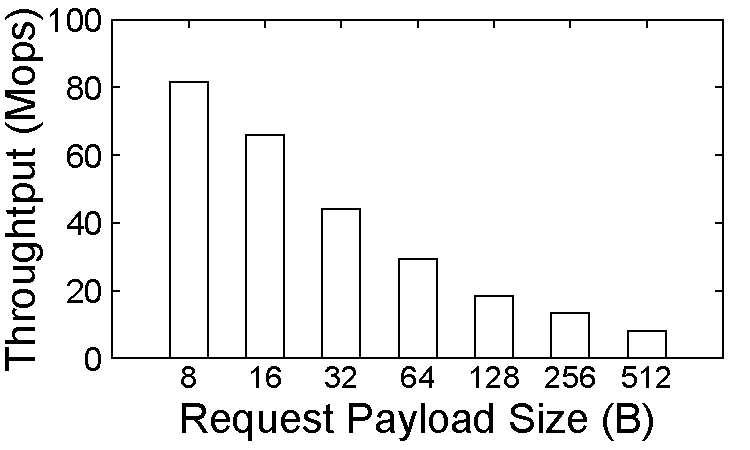
\includegraphics[width=.25\textwidth,page=1]{cpu_random_mem_single_core.pdf}}
\subfloat[Multiple cores.\label{fig:cpu-mem-multi}]
{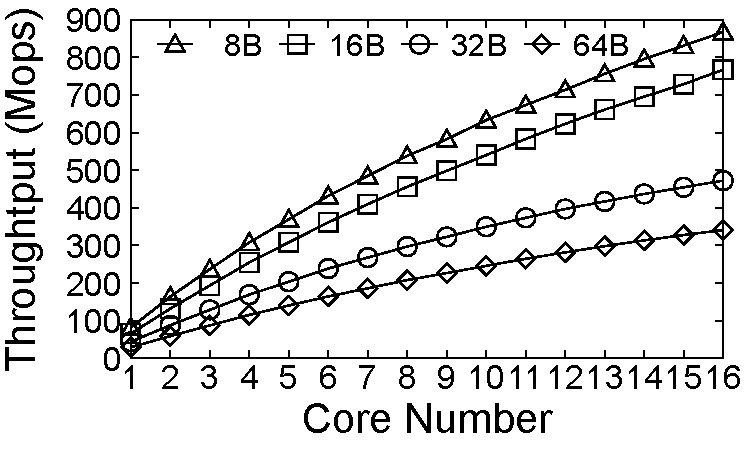
\includegraphics[width=.25\textwidth,page=1]{cpu_random_mem_multi_core.pdf}}
\caption{CPU random memory access performance.}
\label{fig:cpu-mem}
\end{figure}

The latency for CPU to access DRAM on the same NUMA node, \ie cache miss latency, is 80\approx90 nanoseconds on our platform (measured with~\cite{intelmemaccess}, hardware details in sec. \ref{sec:implementation}).
For 64-byte access granularity, the random read latency including data copy is \approx110~ns.
This latency can be partially hidden by the out-of-order execution engine in modern CPUs, which can issue a few memory accesses in parallel.
However, the parallelism is limited by two factors: the number of load-store units (LSUs) per core~\emph{k} (measured to be 3\approx4 on our CPU) and the instruction window size~\emph{W} (measured to be 100\approx200 instructions on our CPU)~\cite{gharachorloo1992hiding, han2010packetshader, zhang2015mega}. When there are enough memory operations in the instruction window, \emph{k} of them can be issued simultaneously. 

\begin{table}[htbp]
\footnotesize
\centering
\label{tab:tput-unroll}
\begin{tabular}{|c|c|c|c|c|c|c|}
\hline
\multirow{2}{*}{Size (B)} & \multirow{2}{*}{CalcOnly} & \multirow{2}{*}{MemOnly} & \multicolumn{4}{c|}{Calc + Mem (Batch Factor)} \\\cline{4-7} 
  &  & & 1 & 2 & 3 & 4 \\\hline
32 & 24.1 & 44.0 & 7.5 & 11.1 & 13.1 & 14.1 \\\hline
64 & 11.1 & 29.3 & 5.5 & 6.7 & 7.6 & 7.9 \\\hline
128 & 5.4 & 18.3 & 3.5 & 4.1 & 4.3 & 4.1 \\\hline
256 & 2.7 & 13.2 & 2.1 & 2.2 & 2.2 & 2.1 \\\hline
512 & 1.3 & 8.2 & 1.2 & 1.1 & 1.2 & 1.1 \\\hline
\end{tabular}
\caption{Throughput (M op/s) under different workload and payload sizes of memory access.}
\label{tab:kv-cpu-throughput}
\end{table}

Figure~\ref{fig:cpu-mem} shows random memory access performances of a multicore CPU. It shows that a modern CPU core can provide fairly high random memory access throughput (27M~op/s or 1.7~GB/s for 64B granularity). Moreover, memory throughput scales linearly with number of CPU cores, indicating that the DDR main memory is not a bottleneck.

However, in a KV store memory access is interleaved with computation for hash slot calculation and key comparison. An operation to access a 64-byte KV pair typically requires \approx100 ns computation or \approx500 instructions, which is far larger than the instruction window size.
Consequently, when the random memory access instructions for different keys are separated by computation, the second DRAM access is too far to fit in the same instruction window with the first DRAM access and cannot be issued in parallel.

One can batch memory accesses in a KV store, i.e. clustering the computation for several operations together before issuing the memory access all at once~\cite{li2016full, narula2014phase}.
Table~\ref{tab:kv-cpu-throughput} depicts the measured per-core hash table throughput under different KV sizes and batch sizes, assuming the KV is inlined in hash table and each KV operation requires one non-cached memory access.
The results fit the following formulas within 10\% error:
\begin{equation}
%\small
\frac{1}{RandAccessThroughput} = \frac{MemLatency}{Parallelism}
\end{equation}
\begin{equation}
%\small \frac{1}{KVThroughput} = ComputeTime + \frac{MemLatency}{min(BatchSz, Parallelism)}
\begin{aligned}
\frac{1}{KVopThroughput} = & ComputationTime + \\
      & \frac{MemLatency}{min(BatchSize, Parallelism)}
\end{aligned}
\end{equation}
This indicates that when interleaved with computation, the performance of CPU degrades significantly. In the extreme case, even if the instruction window size or memory fetch parallelism goes to infinity, the per-core KV operation throughput would still be bounded by computation (\approx10M~op/s), 10\approx20x slower than a single DDR channel.
\end{comment}

\egg{
\subsection{Domain-Specific Architectures for KVS}

Ten years ago, processor frequency scaling was over and people turned to multi-core and concurrency~\cite{sutter2005free}.
Nowadays, CMOS feature-size reduction is getting more and more difficult, which implies that multi-core scaling is also over. People are turning to domain-specific architectures (DSAs)~\cite{esmaeilzadeh2013power} for better performance. Several such DSAs have been used to improve KVS performances. 

\egg{
For computation, DSAs such as GPU, 
FPGA~\cite{putnam2014programmable, caulfield2016cloud} and ASIC~\cite{liu2016cambricon, tpu} have been quickly accepted by the market.
For networking, DSAs are also deployed at scale in datacenters, such as RDMA/RoCE NICs~\cite{mellanoxrdma}, programmable NICs~\cite{greenberg2015sdn, li2016clicknp} and programmable switches~\cite{bosshart2013forwarding}.
}

\subsubsection{One-sided RDMA}

Due to high overhead in CPU network processing, DSAs to accelerate networking, such as RDMA/RoCE NICs~\cite{mellanoxrdma}, are deployed at scale in datacenters. High performance KVS systems can leverage RDMA capable hardware. One approach is to accelerate RPC with \textit{two-sided} verbs in RDMA/RoCE NICs (section \ref{sec:ReduceNetworkingOverhead}, Figure~\ref{fig:memaccess-a}).
By doing so, the KV performance is bounded by CPU (section \ref{sec:CPU-KV-Bottleneck}).

A significantly different approach is to leverage \textit{one-sided} RDMA to access remote memory via the NIC on the client and bypass the CPU on the server, as shown in Figure~\ref{fig:memaccess-b}.
In this approach, KV computation and synchronization are handled by the client CPU, therefore making the KV server very light-weight and high performance.
Despite the high message rate (8M\approx150M~op/s~\cite{kalia2016design}) provided by RDMA NICs, it is challenging to find an efficient match between RDMA primitives and key-value operations.
For a write (PUT or atomic) operation, multiple network round-trips and memory accesses may be required to handle hash conflicts, memory allocation and fetch/save non-inline data.
RDMA does not support transactions. Clients must synchronize with each other to ensure consistency by either using RDMA atomics or distributed atomic broadcast~\cite{szepesi2014designing}, both incurring communication overhead and synchronization latency~\cite{mitchell2013using, dragojevic2014farm}.
As a consequence, most RDMA-based KVS, \eg, Pilaf~\cite{mitchell2013using}, FaRM~\cite{dragojevic2014farm} and HERD~\cite{kalia2014using} recommend using one-sided RDMA for GET operations only. For PUT operations, they fall back to two-sided RDMA as RPC and let the remote CPU do the actual work. Throughput of write-intensive workload is still bottlenecked by CPU cores.

In addition to the mismatch between RDMA primitives and KV operations, implementation of commodity RDMA NICs also constrain KV throughput. For example, RDMA NICs hold a lock for atomic operations when a PCIe DMA to the same memory address is in flight, which bounds RDMA atomics throughput to \approx2M~op/s~\cite{kalia2016design}.

\subsubsection{Highly parallel architectures}

Highly parallel architectures such as many-core processors~\cite{berezecki2011many}, GPGPU~\cite{zhang2015mega}.

\subsubsection{FPGA}

FPGA~\cite{istvan2013flexible, chalamalasetti2013fpga, maohardware, lavasani2014fpga, istvan2015hash, istvan2016consensus, kvs-openpower, istvan2015hash, sidler2015scalable, blott2015scaling} have been explored to overcome the limited parallelism of CPU in accessing DRAM.
Compared to general-purpose processors, FPGA has more flexible pipeline parallelism and can be specialized for the key-value store application.
Compared to RDMA, FPGA can support key-value operation primitives directly, as well as specializing network packet format and PCIe DMA operations to use network and PCIe bandwidth efficiently.
Compared to GPGPU, FPGA is more power-efficient and has lower latency.

In recent years, FPGA is becoming cost-effective and is getting deployed at scale in datacenters~\cite{putnam2014programmable, caulfield2016cloud}. Its programmability has been greatly improved~\cite{li2016clicknp}.
Most existing work store the entire hash table inside the on-board DRAM, which is often quite limiting (typically on the order of 4\approx16~GiB), while the host DRAM is often large (on the order of 100\approx500~GiB).
KV-Direct follows this line of work, while leveraging host DRAM for KV storage, as depicted in Figure~\ref{fig:memaccess-c}.

KV-Direct leverages a programmable NIC with large-scale deployments in datacenters.
The programmable NIC is composed of two parts: a traditional RDMA NIC plus a field-programmable gate array (FPGA).
There has been research on leveraging the reconfigurability of the NIC for network processing, \eg, network virtualization~\cite{greenberg2015sdn, vfp} and network functions~\cite{li2016clicknp}.
KV-Direct extends the application of programmable NICs to a novel area: key-value stores.
}

\subsection{Workload Shift in KVS}
\label{sec:workload-shift}

Historically, KVS such as Memcached~\cite{fitzpatrick2004distributed} gained popularity as an object caching system for web services.
In the era of in-memory computation, KVS goes beyond caching and becomes an infrastructure service to store shared data structure in a distributed system.
Many data structures can be expressed in a key-value hash table, \eg, data indexes in NoSQL databases~\cite{chang2008bigtable}, model parameters in machine learning~\cite{li2014scaling}, nodes and edges in graph computing~\cite{shao2013trinity, xiao17tux2} and sequencers in distributed synchronization~\cite{kalia2016design}.

The workload shifts from object cache to generic data structure store implies several design goals for KVS.

\textbf{High batch throughput for small KV.}
In-memory computations typically access small key-value pairs in large batches, \eg, sparse parameters in linear regression~\cite{li2014algorithmic, xiao17tux2} or all neighbor nodes in graph traversal~\cite{shao2013trinity}, therefore a KVS should be able to benefit from batching and pipelining.
%If the throughput of remote key-value access is comparable to accessing a local hash table, distributed computation on shared memory could be easier to scale linearly.

\textbf{Predictable low latency.}
For many data-parallel computation tasks, the latency of an iteration is determined by the slowest operations~\cite{ousterhout2015ramcloud}. Therefore, it is important to control the tail latency of KVS. CPU based implementations often have large fluctuations under heavy load due to scheduling irregularities and inflated buffering.
%CPU-based designs may need to trade-off latency and throughput by adjusting batch size~\cite{li2016full}, while hardware-accelerated designs can leverage pipelining to boost throughput without sacrificing latency~\cite{kalia2016design}.
%Additionally, CPU processing time may have large fluctuations under high load due to scheduling irregularities, while hardware pipelines often have stable latency~\cite{li2016clicknp}.

\textbf{Efficient under the write-intensive workload.}
For cache workloads, KVS often has much more reads than writes~\cite{atikoglu2012workload}, but it is no longer the case for distributed computation workloads
such as graph computation~\cite{page1999pagerank} and parameter servers~\cite{li2014scaling}.
%For PageRank computation in a graph~\cite{page1999pagerank} or gradient descent in parameter servers~\cite{li2014scaling}, each node or parameter is read and written once per iteration, and the KVS would serve an equal number of GET and PUT operations.
%Sequencers~\cite{kalia2016design} require atomic increment operations and no read-only operations.
These workloads favor hash table structures that can handle both read and write operations efficiently.


\textbf{Fast atomic operations.}
Atomic operations on several extremely popular keys appear in applications such as centralized schedulers~\cite{perry2014fastpass}, sequencers~\cite{kalia2016design}, counters~\cite{zhu2015packet} and short-term values in web applications~\cite{atikoglu2012workload}.
This requires high throughput on single-key atomics.
%CPU-based KVS atomics is bottlenecked by either core contention or per-core throughput~\cite{li2016full}, and atomics based on one-sided RDMA is bottlenecked by PCIe latency~\cite{kalia2016design}.

\textbf{Support vector type operations.}
Machine learning and graph computing workloads~\cite{li2014scaling,shao2013trinity,xiao17tux2} often require operating on every element in a vector,
\eg, incrementing every element in a vector with a scalar or reducing a vector into the sum of its elements.
KVS without vector support requires the client to either issue one KVS operation per element, or retrieve the vector back to the client and perform the operation.
Supporting vector data type and operations in KVS can greatly reduce network communication and CPU computation overhead.


\subsection{Achilles' Heel of High-Performance KVS Systems}
\label{sec:state-of-the-art-kvs}

Building a high performance KVS is a non-trivial exercise of optimizing various software and hardware components in a computer system.
Characterized by where the KV processing takes place, state-of-the-art high-performance KVS systems basically falls into three categories:
on the CPU of KVS server
%~\cite{mao2012cache,fan2013memc3,li2014algorithmic,ousterhout2010case, ousterhout2015ramcloud, kapoor2012chronos, lim2014mica,li2016full,kalia2014using, kalia2016design}
(Figure~\ref{fig:memaccess-a}),
on KVS clients
%~\cite{mitchell2013using,szepesi2014designing,dragojevic2014farm,kalia2014using}
(Figure~\ref{fig:memaccess-b})
or on a hardware accelerator
%~\cite{zhang2015mega,berezecki2011many,liang16fpl,blott13hotcloud,lavasani2014fpga,chalamalasetti2013fpga}
(Figure~\ref{fig:memaccess-c}).

When pushed to the limit, in high performance KVS systems the throughput bottleneck can be attributed to the computation in KV operation and the latency in random memory access.
CPU-based KVS needs to spend CPU cycles for key comparison and hash slot computation.
Moreover, KVS hash table is orders of magnitude larger than the CPU cache, therefore the memory access latency is dominated by cache miss latency for practical access patterns.

\begin{itemize}
\item 
\begin{itemize}
\item 
\end{itemize}
\end{itemize}
By our measurement, a 64-byte random read latency for a contemporary computer is \approx110~ns. A CPU core can issue several memory access instructions concurrently when they fall in the instruction window, limited by the number of load-store units in a core (measured to be 3\approx4 in our CPU)~\cite{gharachorloo1992hiding, han2010packetshader, zhang2015mega}. In our CPU, we measure a max throughput of 29.3~M random 64B access per second per core. On the other hand, an operation to access 64-byte KV pair typically requires \approx100~ns computation or \approx500 instructions, which is too large to fit in the instruction window (measured to be 100\approx200). When interleaved with computation, the performance of a CPU core degrades to only 5.5~M KV operations per second (Mops). An optimization is to batch memory accesses in a KV store by clustering the computation for several operations together before issuing the memory access all at once~\cite{li2016full, narula2014phase}. This improves the per-core throughput to 7.9~MOps in our CPU, which is still far less than the random 64B throughput of host DRAM.

Observing the limited capacity of CPU in KV processing, recent work~\cite{mitchell2013using,szepesi2014designing,dragojevic2014farm} leverage one-sided RDMA to offload KV processing to clients and effectively using the KVS server as a shared memory pool.
Despite the high message rate (8\approx150~Mops~\cite{kalia2016design}) provided by RDMA NICs, it is challenging to find an efficient match between RDMA primitives and key-value operations.
For a write (PUT or atomic) operation, multiple network round-trips and multiple memory accesses may be required to query the hash index, handle hash collisions and allocate variable-size memory.
RDMA does not support transactions. Clients must synchronize with each other to ensure consistency using RDMA atomics or distributed atomic broadcast~\cite{szepesi2014designing}, both incurring communication overhead and synchronization latency~\cite{mitchell2013using, dragojevic2014farm}.
Therefore, most RDMA-based KVS~\cite{mitchell2013using,dragojevic2014farm,kalia2014using} recommend using one-sided RDMA for GET operations only. For PUT operations, they fall back to the server CPU. The throughput of write-intensive workload is still bottlenecked by CPU cores.

\subsection{Programmable NIC with FPGA}
\label{sec:programmable-nic}

\begin{figure}[t]
\centering
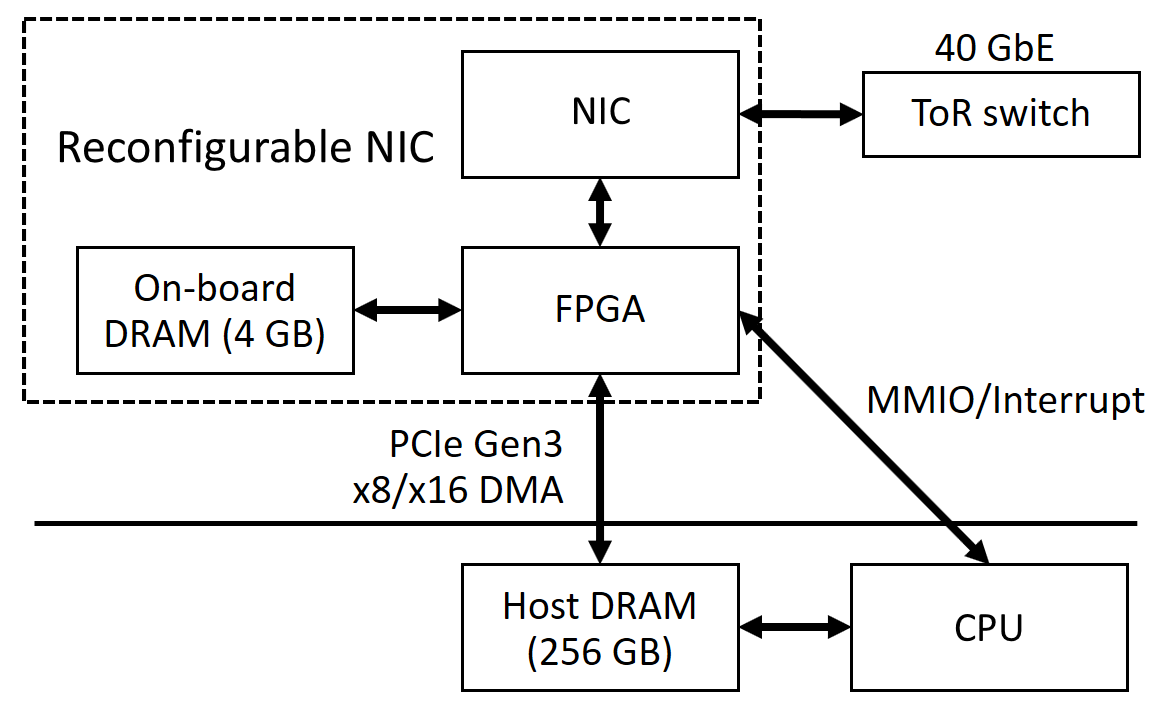
\includegraphics[width=0.33\textwidth]{sys_architecture.PNG}
\caption{Programmable NIC with FPGA.}
\label{fig:kvdirect-arch}
\vspace{-15pt}
\end{figure}

Ten years ago, processor frequency scaling slowed down and people turned to multi-core and concurrency~\cite{sutter2005free}.
Nowadays, power ceiling implies that multi-core scaling has also met difficulties~\cite{esmaeilzadeh2013power}.
People are now turning to domain-specific architectures (DSAs) for better performance.

%On the spectrum of hardware programmability and performance, general-purpose processors lie on the programmability end, while application-specific integrated circuits (ASICs) lie on the performance end.
%Field-programmable gate array (FPGA) is an architecture between the two extremes, providing both programmability and performance~\cite{bacon2013fpga}.
%As its name indicates, FPGA is a sea of gates.
%Millions of reconfigurable gates and thousands of small block RAMs (BRAMs) provide massive parallelism to build thousands of ``cores'' running simultaneously, and more importantly, customized interconnections among the ``cores'' and BRAMs specializing communication and synchronization for a certain application.
%Consequently, for applications with sufficient bit-level and task-level parallelism, FPGAs provide not only high throughput and power efficiency, but also low and predictable latency.

Due to the increasing mismatch of network speed and CPU network processing capacity, programmable NICs with FPGA now witness large-scale deployment in datacenters~\cite{vfp,greenberg2015sdn,li2016clicknp}.
As shown in Figure~\ref{fig:kvdirect-arch}, the heart of the programmable NIC we use~\cite{li2016clicknp} is an FPGA, with an embedded NIC chip to connect to the network.
Programmable NICs typically come with on-board DRAM as packet buffers and runtime memory for NIC firmware~\cite{putnam2014reconfigurable,li2016clicknp}.

\subsection{Challenges for Remote Direct Key-Value Access}
\label{sec:challenge}

\begin{figure}[t]
\centering
\subfloat[Throughput.\label{fig:dma-tput}]
{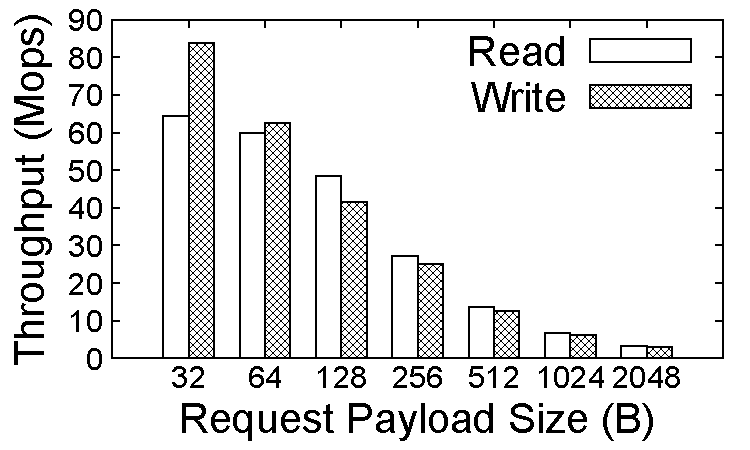
\includegraphics[width=.25\textwidth,page=1]{pcie_bw.pdf}}
\subfloat[DMA Read Latency.\label{fig:dma-lat}]
{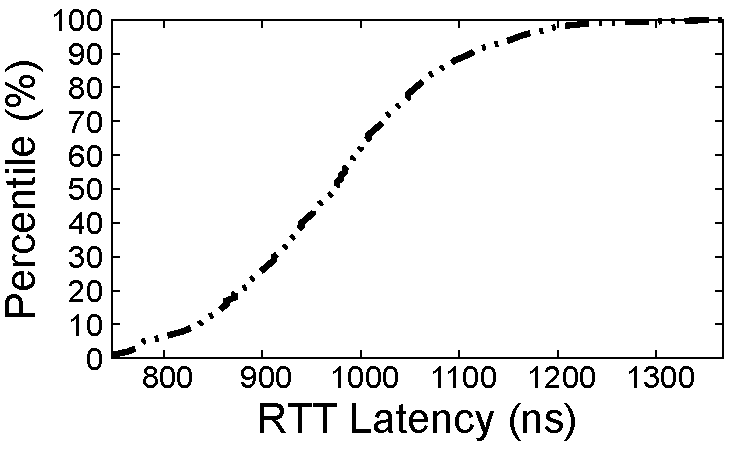
\includegraphics[width=.25\textwidth,page=1]{pcie_latency.pdf}}
\caption{PCIe random DMA performance.}
\label{fig:dma-perf}
\vspace{-10pt}
\end{figure}

KV-Direct moves KV processing from the CPU to the programmable NIC in the server (Figure~\ref{fig:memaccess-c}).
Same as RDMA, the KV-Direct NIC accesses host memory via PCIe. PCIe is a packet switched network with \approx500~ns round-trip latency and 7.87~GB/s theoretical bandwidth per Gen3 x8 endpoint.
On the latency side, for our programmable NIC, the cached PCIe DMA read latency is 800~ns due to additional processing delay in FPGA.
For random non-cached DMA read, there is an additional 250~ns average latency (Figure~\ref{fig:dma-lat}) due to DRAM access, DRAM refresh and PCIe response reordering in PCIe DMA engine.
On the throughput side, each DMA read or write operation needs a PCIe transport-layer packet (TLP) with 26-byte header and padding for 64-bit addressing.
For a PCIe Gen3 x8 NIC to access host memory in 64-byte granularity, the theoretical throughput is therefore 5.6~GB/s, or 87~Mops.

To saturate PCIe Gen3 x8 with 64-byte DMA requests, 92 concurrent DMA requests are needed considering our latency of 1050~ns.
In practice, two factors further limit the concurrency of DMA requests.
First, PCIe credit-based flow control constrains the number of in-flight requests for each DMA type. The PCIe root complex in our server advertises 88 posted header credits for DMA write and 84 non-posted header credits for DMA read.
Second, DMA read requires assigning a unique PCIe tag to identify DMA responses which may come out of order.
The DMA engine in our FPGA only support 64 PCIe tags, further limiting our DMA read concurrency to 64 requests, which renders a throughput of 60~Mops as shown in Figure~\ref{fig:dma-tput}.
On the other hand, with 40~Gbps network and 64-byte KV pairs, the batch throughput roof is 78Mops.
In order to saturate the network, the KVS on NIC must make full use of PCIe bandwidth and have close to one average memory access per small GET or PUT.
This boils down to three challenges:

\textbf{Minimize DMA requests per KV operation.}
Hash table and memory allocation are two major components in KVS that require random memory access.
Previous works propose hash tables~\cite{dragojevic2014farm, breslow2016horton} with close to 1 memory access per GET operation even under high load factors.
However, under $>$50\% load factor, these tables need multiple memory accesses per PUT operation on average with large variance.
This not only consumes PCIe throughput, but also leads to latency variations for write-intensive workloads.

In addition to hash table lookup, dynamic memory allocation is required to store variable-length KVs that cannot be inlined in the hash table.
Minimizing hash table lookups per KV operation and memory accesses per memory allocation is essential for matching PCIe and network throughput under write-intensive, small-KV workloads.

\textbf{Hide PCIe latency while maintaining consistency.}
An efficient KVS on NIC must pipeline KV operations and DMA requests to hide the PCIe latency.
However, KV operations may have dependencies.
A GET following PUT on a same key needs to return the updated value.
%Two adjacent atomic add operations needs to wait for the first to finish before executing the second.
This requires tracking KV operations being processed and stall the pipeline on data hazard, or better, design an out-of-order executor to resolve data dependency without explicitly stalling the pipeline.


\textbf{Leverage on-board DRAM.}
%Currently the DRAM is underutilized both in terms of space and throughput.
An obvious idea is to use the on-board DRAM as cache for host memory, but the DRAM throughput (12.8~GB/s) is less than the achievable throughput (13.2~GB/s) of two PCIe Gen3 x8 endpoints in our NIC.
It is more desirable to distribute memory access between DRAM and host memory in order to utilize both of their bandwidths.
However, the on-board DRAM is small (4~GiB) compared to the host memory (64~GiB), calling for a hybrid caching and load-dispatching approach.

In the following, we will present KV-Direct, a novel FPGA-based key-value store that satisfies all aforementioned goals and describe how we address the challenges.
1
\section{Design}
\label{sec:architecture}

\subsection{System Architecture}

KV-Direct enables \textit{remote direct key-value access}.
Clients send \textit{KV-Direct operations} (\S\ref{sec:kv-operations}) to KVS server while the \ournic{} processes the requests and sending back results, bypassing the CPU.
-The \ournic{} on KVS server is an FPGA reconfigured as a \textit{KV processor} (\S\ref{sec:kv-processor}).
Figure~\ref{fig:kvdirect-arch} shows the architecture of KV-Direct.

\subsection{KV-Direct Operations}
\label{sec:kv-operations}

\begin{table}
\centering
\caption{KV-Direct operations.}
\label{tab:kv-operations}
\small
\begin{tabular}{p{.16\textwidth}|p{.28\textwidth} }
\toprule
get ($k$) $\rightarrow v$ & Get the value of key $k$. \\
\midrule
put ($k, v$) $\rightarrow$ bool & Insert or replace a $(k, v)$ pair. \\
\midrule
delete ($k$) $\rightarrow$ bool & Delete key $k$. \\
\midrule
\midrule
update{\_}scalar2scalar ($k, \Delta, \lambda(v, \Delta) \rightarrow v$) $\rightarrow v$ & Atomically update the value of key~$k$ using function~$\lambda$ on scalar~$\Delta$, and return the original value. \\
\midrule
update{\_}scalar2vector ($k, \Delta, \lambda(v, \Delta) \rightarrow v$) $\rightarrow [v]$ & Atomically update all elements in vector~$k$ using function~$\lambda$ and scalar~$\Delta$, and return the original vector. \\
\midrule
update{\_}vector2vector ($k, [\Delta], \lambda(v, \Delta) \rightarrow v$) $\rightarrow [v]$ & Atomically update each element in vector~$k$ using function~$\lambda$ on the corresponding element in vector~$[\Delta]$, and return the original vector. \\
\midrule
reduce ($k, \Sigma, \lambda(v, \Sigma) \rightarrow \Sigma$) $\rightarrow \Sigma$ & Reduce vector~$k$ to a scalar using function~$\lambda$ on initial value, and return the reduction result~$\Sigma$. \\
\midrule
filter ($k, \lambda(v) \rightarrow$ bool) $\rightarrow [v]$ & Filter elements in a vector~$k$ by function~$\lambda$, and return the filtered vector. \\
\bottomrule
\end{tabular}
\vspace{-10pt}
\end{table}

KV-Direct extends one-sided RDMA operations to key-value operations, as summarized in Table~\ref{tab:kv-operations}.
In addition to standard KVS operations as shown in the top part of Table~\ref{tab:kv-operations}, KV-Direct supports vector operations, as well as \textit{active messages}~\cite{eicken1992active} as a generalization to atomic operations.
Active messages enable near-memory computation and save communication and synchronization cost.

When a vector operation update, reduce or filter is operated on a key, its value is treated as an array of fixed-bit-width elements.
Each function $\lambda$ operates on one element in the vector, a client-specified parameter~$\Delta$, and/or an initial value~$\Sigma$ for reduction.
For efficiency, the $\lambda$ functions are compiled into hardware logic, so they need to be pre-registered by the KVS client and substituted with numeric opcodes during runtime.
The KV-Direct development toolchain duplicates the $\lambda$ several times to leverage parallelism in FPGA and match computation throughput with PCIe throughput, then compiles it into hardware logic using an high-level synthesis (HLS) tool~\cite{aoc}.
The HLS tool automatically extracts data dependencies in the duplicated function and generates a fully pipelined programmable logic.
%Before executing the KVS client, the programmable NIC on KVS servers should be loaded with the hardware logic containing the unrolled $\lambda$.

Update operations with active messages not only cover standard scalar atomic operations such as compare-and-swap and fetch-and-add, but also capable of general stream processing on a vector value.
For example, a network processing application may interpret the vector as a stream of packets for network functions~\cite{li2016clicknp} or a bunch of states for packet transactions~\cite{sivaraman2016packet}.
Single-object transaction processing completely in the programmable NIC is also possible, \eg, wrapping around S\_QUANTITY in TPC-C benchmark~\cite{council2010tpc}.
Vector reduce operation supports neighbor weight accumulation in PageRank~\cite{page1999pagerank}.
Non-zero values in a sparse vector can be fetched efficiently with vector filter operation.

\subsection{KV Processor}
\label{sec:kv-processor}

\begin{figure}[t]
\centering
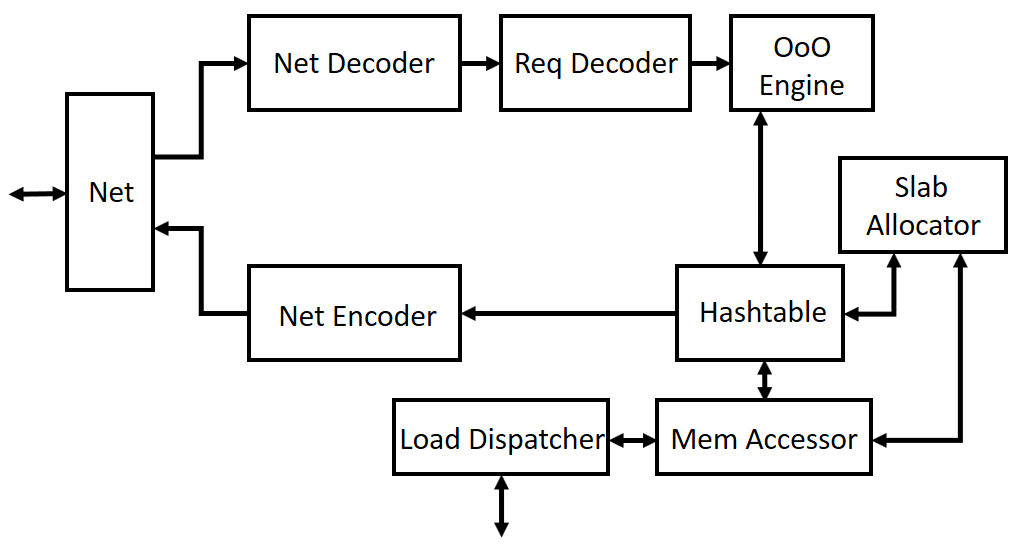
\includegraphics[width=0.4\textwidth,page=1]{processor_architecture.PNG}
\caption{KV processor architecture.}
\label{fig:kvprocessor-arch}
\vspace{-10pt}
\end{figure}

As shown in Figure~\ref{fig:kvprocessor-arch}, the KV processor receives packets from the on-board NIC, decodes vector operations and buffers KV operations in the reservation station (\S\ref{sec:ooo}).
Next, the out-of-order engine (\S\ref{sec:ooo}) issues independent KV operations from reservation station into the operation decoder.
Depending on the operation type, the KV processor looks up the hash table (\S\ref{sec:hashtable}) and executes the corresponding operations.
To minimize the number of memory accesses, small KV pairs are stored \textit{inline} in the hash table, others are stored in dynamically allocated memory from the slab memory allocator (\S\ref{sec:slab}).
Both the hash index and the slab-allocated memory are managed by a unified memory access engine (\S\ref{sec:dram-cache}), which accesses the host memory via PCIe DMA and caches a portion of host memory in on-board DRAM.
After the KV operation completes, the result is sent back to the out-of-order execution engine (\S\ref{sec:ooo}) to find and execute matching KV operations in reservation station.

As discussed in \S\ref{sec:challenge}, the scarcity of PCIe operation throughput requires the KV processor to be frugal on DMA accesses.
For GET operation, at least one memory read is required.
For PUT or DELETE operation, one read and one write are minimal.
KV-Direct carefully designs the hash table to achieve close to ideal DMA accesses per lookup and insertion, as well as the memory allocator to achieve $<$~0.1 amortized DMA operations per dynamic memory allocation.

\subsubsection{Hash Table}
\label{sec:hashtable}

\begin{figure}[t]
\centering
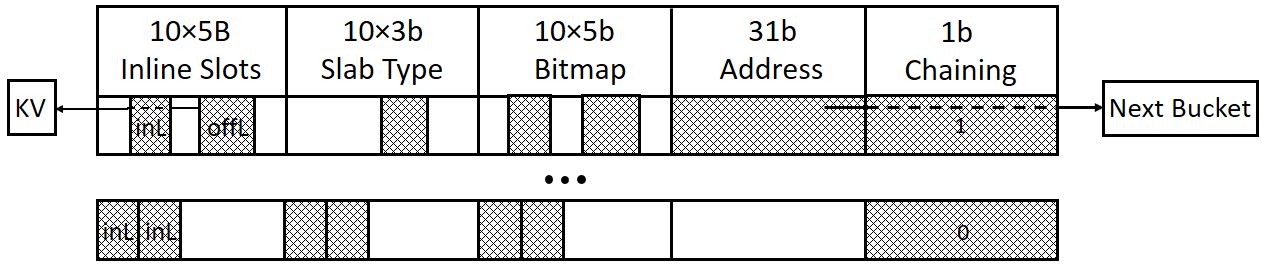
\includegraphics[width=.5\textwidth,page=1]{hashline.PNG}
\caption{Hash index structure. Each line is a hash bucket containing 10 hash slots, 3 bits of slab memory type per hash slot, one bitmap marking the beginning and end of inline KV pairs and a pointer to the next chained bucket on hash collision.}
\label{fig:hashtable}
\vspace{-10pt}
\end{figure}

To store variable-sized KVs, the KV storage is partitioned into two parts. The first part is a hash index (Figure~\ref{fig:hashtable}), which consists a fixed number of \textit{hash buckets}. Each hash bucket contains several \textit{hash slots} and some metadata. The rest of the memory is dynamically allocated, and managed by a slab allocator (\S\ref{sec:slab}).
A \textit{hash index ratio} configured at initialization time determines the percentage of the memory allocated for hash index.
The choice of hash index ratio will be discussed in \S\ref{sec:hashtable-eval}.

%\textbf{Hash Table.}
%Each bucket includes 10 hash slots, 3b type code per slot, 50b metadata, plus 31b address and a valid bit of the next chained bucket, as shown in Figure~\ref{fig:hashtable}.
%For offline KVs, each hash slot needs to store 31b of address, 9b of secondary hash and 3b type code for the slab size.
%For inline KVs, to mark the begin and end of each hash slot, as well as the separation between inline key and value, the information is encoded in a 50b metadata corresponding to 50 bytes of hash slots.
%The inline keys and secondary hashes of offline keys in all hash slots are compared in parallel, and the first match is found.

Each hash slot includes a pointer to the KV data in dynamically allocated memory and a secondary hash for quick probabilistic comparison.
Assuming a 64~GiB KV storage in host memory and 32-byte allocation granularity, the pointer requires 31 bits.
A secondary hash of 9 bits gives a 1/512 false positive possibility.
Cumulatively, the hash slot size is 5 bytes.
To determine the hash bucket size, we need to trade-off between the number of hash slots per bucket and the DMA throughput.
Figure~\ref{fig:dma-tput} shows that the DMA read throughput below 64B granularity is bound by PCIe latency and parallelism in the DMA engine.
A bucket size less than 64B is suboptimal due to increased possibility of hash collision.
On the other hand, increasing the bucket size above 64B would decrease hash lookup throughput.
So we choose the bucket size to be 64 bytes.

\begin{figure}[t]
\centering
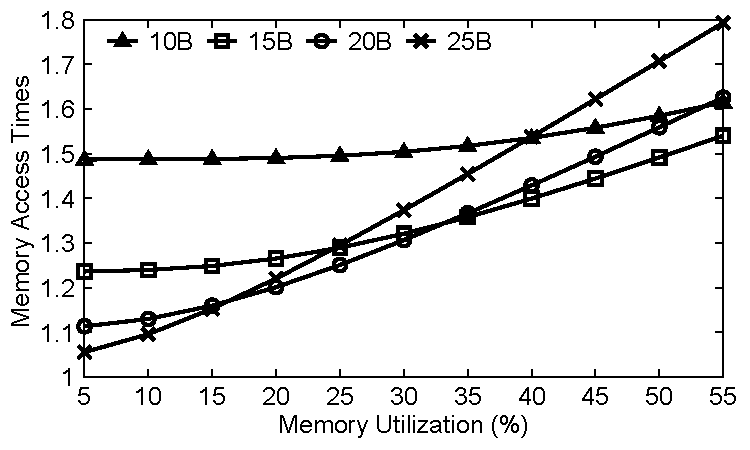
\includegraphics[width=0.33\textwidth]{inline_thresh.pdf}
\caption{Average memory access count under varying inline thresholds (10B, 15B, 20B, 25B) and memory utilizations.}
\label{fig:inline-offline}
\vspace{-10pt}
\end{figure}

Small KVs are stored \textit{inline} in the hash index to save the additional memory access to fetch KV data.
An inline KV may span multiple hash slots.
It might not be optimal to inline all KV that can fit in a bucket.
To minimize average access time, assuming that smaller and larger keys are equally likely to be accessed, it is more desirable to inline KVs smaller than an \textit{inline threshold}.
As shown in Figure~\ref{fig:inline-offline}, for a certain inline threshold, the average memory access count increases with memory utilization, due to more hash collisions.
Higher inline threshold shows a more steep growth curve of memory access count, so an optimal inline threshold can be found to minimize memory accesses under a given memory utilization.
As with hash index ratio, the inline threshold can also be configured at initialization time.

When all slots in a bucket are filled up, there are several solutions to resolve hash collisions.
Cuckoo hashing~\cite{pagh2004cuckoo} and hopscotch hashing~\cite{herlihy2008hopscotch} achieve constant-time lookup by moving occupied slots during insertion.
In write-intensive workload, the memory access time under high load factor would experience large fluctuations.
Linear probing may suffer from primary clustering, therefore its performance is sensitive to the uniformity of hash function.
We choose \textit{chaining} to resolve hash conflicts, which balances lookup and insertion, while being more robust to hash clustering.


%In KV-Direct, we measure memory utilization instead of load factor, because chaining has dynamic size and that we care more about the overall storage efficiency counting all indexing, metadata and memory fragmentation overhead.
%Clearly, small KVs cause lower memory utilization due to metadata overhead.
%The optimal hash index ratio is chosen at initialization time according to workload to balance average access time and memory utilization.

\subsubsection{Slab Memory Allocator}
\label{sec:slab}

Chained hash slots and non-inline KVs need dynamic memory allocation.
We choose slab memory allocator~\cite{bonwick1994slab} to achieve $O(1)$ average memory access per allocation and deallocation. The main slab allocator logic runs on host CPU and communicates with the KV-processor through PCIe.
Slab allocator rounds up allocation size to the nearest power of two, called \textit{slab size}.
It maintains a \textit{free slab pool} for each possible slab size (32, 64, \ldots, 512 bytes), and a global \textit{allocation bitmap} to help to merge small free slabs back to larger slabs.
Each free slab pool is an array of \textit{slab entries} consisting of an address field and a slab type field indicating the size of the slab entry.
The free slab pool can be cached on the NIC. The cache syncs with the host memory in batches of slab entries. Amortized by batching, less than 0.07 DMA operation is needed per allocation or deallocation.
When a small slab pool is almost empty, larger slabs need to be split.
Because the slab type is already included in a slab entry, in \textit{slab splitting}, slab entries are simply copied from the larger pool to the smaller pool, without the need for computation.
Including slab type in the slab entry also saves communication cost because one slab entry may contain multiple slots.

On deallocation, the slab allocator needs to check whether the freed slab can be merged with its neighbor, requiring at least one read and write to the allocation bitmap.
Inspired by garbage collection, we propose \textit{lazy slab merging} to merge free slabs in batch when a slab pool is almost empty and no larger slab pools have enough slabs to split.

\subsubsection{Out-of-Order Execution Engine}
\label{sec:ooo}
%
%\begin{figure}[t]
%\centering
%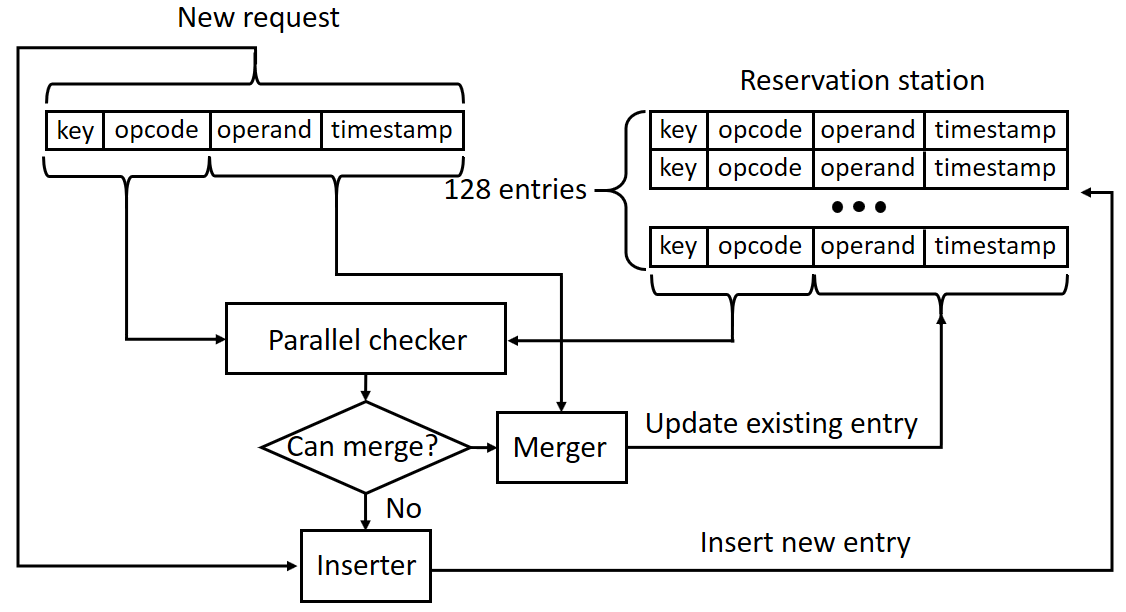
\includegraphics[width=.45\textwidth,page=1]{dynamic_scheduler.PNG}
%\caption{Dynamic operation scheduler.}
%\label{fig:ooo-mem-access}
%\vspace{-10pt}
%\end{figure}

Dependency between two KV operations with the same key in the KV processor will lead to data hazard and pipeline stall.
This problem is magnified in single-key atomics where all operations are dependent, thus limiting the atomics throughput.
We borrow the concept of dynamic scheduling from computer architecture and implement a \textit{reservation station} to track all in-flight KV operations and their \textit{execution context}.
To saturate PCIe, DRAM and the processing pipeline, up to 256 in-flight KV operations are needed.
However, comparing 256 16-byte keys in parallel would take 40\% logic resource of our FPGA.
Instead, we store the KV operations in a small hash table in on-chip RAM, indexed by the hash of the key.
To simplify hash collision resolution, we regard KV operations with the same hash as dependent, so there may be false positives, but it will never miss a dependency.
Operations with the same hash are organized in a chain and examined sequentially.
Hash collision would degrade the efficiency of chain examination, so the reservation station contains 1024 hash slots to make hash collision possibility below 25\%.

The reservation station not only holds pending operations, but also caches their latest values for \textit{data forwarding}.
When a KV operation is completed by the main processing pipeline, its result is returned to the client, and the latest value is forwarded to the reservation station.
Pending operations in the same hash slot are checked one by one, and operations with matching key are executed immediately and removed from the reservation station.
For atomic operations, the computation is performed in a dedicated execution engine.
For write operations, the cached value is updated.
The execution result is returned to the client directly.
After scanning through the chain of dependent operations, if the cached value is updated, a PUT operation is issued to the main processing pipeline for cache write back.
This data forwarding and fast execution path enable single-key atomics to be processed one operation per clock cycle (180~Mops), eliminate head-of-line blocking under workload with popular keys, and ensure consistency because no two operations on the same key can be in the main processing pipeline simultaneously.


\subsubsection{DRAM Load Dispatcher}
\label{sec:dram-cache}

\begin{figure}[t]
\centering
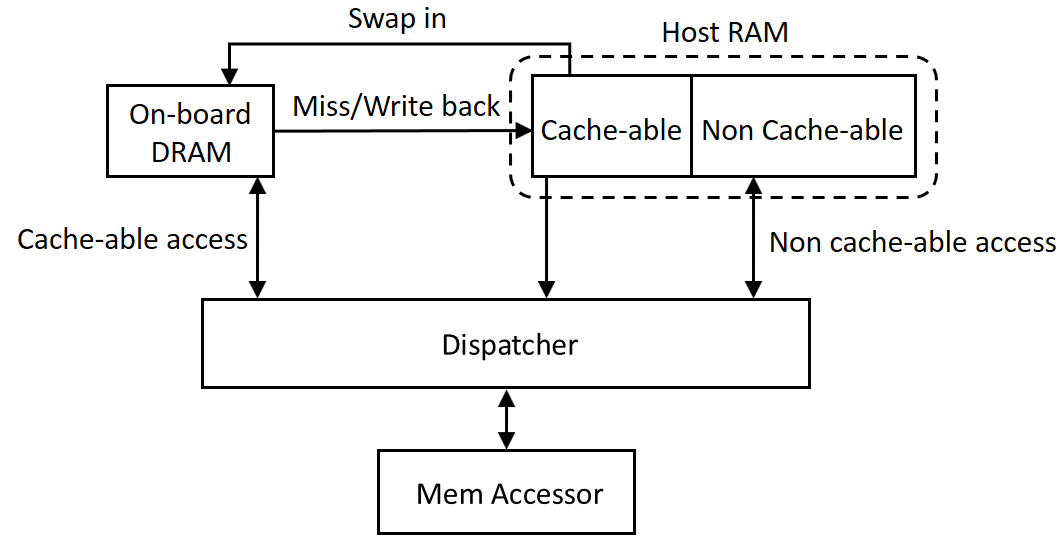
\includegraphics[width=0.4\textwidth,page=1]{load_balancer.PNG}
\caption{DRAM load dispatcher.}
\label{fig:cache}
\vspace{-15pt}
\end{figure}

To further save the burden on PCIe, we dispatch memory accesses between PCIe and the on-board DRAM.
Our on-board DRAM has 4~GiB size and 12.8~GB/s throughput, which is an order of magnitude smaller than the KVS storage on host DRAM (64~GiB) and slightly slower than the PCIe link (14~GB/s).
One approach is to put a fixed portion of the KVS in on-board DRAM. However, the on-board DRAM is too small to carry a significant portion of memory accesses.
The other approach is to use the on-board DRAM as a cache for host memory, the throughput would degrade due to the limited throughput of our on-board DRAM.

We adopt a hybrid solution to use the DRAM as a cache for a fixed portion of the KVS in host memory, as shown in Figure~\ref{fig:cache}.
The portion of cache-able memory in the entire KVS memory is called \textit{load dispatch ratio}.
With a larger load dispatch ratio $l$, more load is dispatched to the on-board DRAM and the cache hit ratio $h(l)$ would increase.
To balance load on PCIe and on-board DRAM, the load dispatch ratio $l$ should be optimized such that:
$$\frac{l}{tput_{DRAM}} = \frac{(1-l) + l \cdot (1-h(l))}{tput_{PCIe}}$$

Specifically, under uniform workload, let $k$ be the ratio of on-board DRAM size and host KV storage size, cache hit ratio $h(l) = k/l$.
Under long-tail workload with Zipf distribution, assume $n$ is the total number of KVs, approximately $h(l) = \frac{\log (kn/l)}{\log n} = \frac{\log kn}{\log n} - \frac{1}{\log n}\log l$.
For these simple key distributions, we can derive a closed form of the optimal load dispatch ratio $l$.



\egg{
\subsubsection{Congestion Avoidance}
\label{sec:congestion-avoidance}

In addition to throughput, another important factor is latency.
From the client's perspective, the KV processor is a path with multiple bottlenecks and buffers, \eg, PCIe and DRAM access.
If all buffers in the KV processor are filled up, the GET latency would exceed 10~$\mu$s.
To mitigate the bufferbloat problem, we implement a congestion avoidance logic to limit the number of in-flight KV operations \textit{inside the KV processor}.
The KV processor maintains a \textit{KV operation window} and leverages credit-based flow control mechanism in RDMA to back-pressure KVS clients.
To adapt KV operation window size to the workload, we measure the running average of KV processing delay and adjust the window size according to TCP Vegas congestion avoidance algorithm~\cite{brakmo1995tcp}.
%We use delay as the congestion signal instead of ECN, because the queues whose sizes are hard to measure.
}

\section{Implementation}
\label{sec:implementation}

Our hardware platform is built on an Intel Stratix V FPGA based programmable NIC (\S\ref{sec:programmable-nic}).
The programmable NIC is attached to the server through two PCIe Gen3 x8 links in a bifurcated x16 physical connector, and contains 4 GiB of on-board DRAM with a single DDR3-1600 channel.

%Predominately, FPGAs are programmed with low-level hardware description languages.
For development efficiency, Intel FPGA SDK for OpenCL~\cite{aoc} as a high-level synthesis tool to generate hardware logic from OpenCL.
Our KV processor is implemented in 11K lines of OpenCL code and all kernels are fully pipelined, \ie, the throughput is one operation per clock cycle.
With 180~MHz clock frequency, our design can process KV operations at 180~M op/s if not bottlenecked by I/O.

%
%\begin{table}[t!]
%	\centering
%	\caption{Line of code and resource utilization of the KV processor.}
%	\label{tab:resource-util}
%	\scalebox{0.8}{
%		\begin{tabular}{l|r|r|r}
%			\toprule
%			Component & LoC & Logic (\%) & Memory (\%) \\
%			\midrule
%            Hash table & & & \\
%            Slab memory allocator & & & \\
%            Dynamic operation scheduler & & & \\
%            DRAM load dispatcher & & & \\
%            Operation decoder & & & \\
%            \midrule
%            Interconnect & & & \\
%            OpenCL runtime & & & \\
%            Network hard IP & & & \\
%            PCIe DMA and hard IP & & & \\
%            DDR controller & & & \\
%            \midrule
%            Total & & & \\
%			\bottomrule
%		\end{tabular}
%	}
%\end{table}


Below highlights two implementation details in the KV processor.


\textbf{Slab Memory Allocator.}

\begin{figure}[t]
\centering
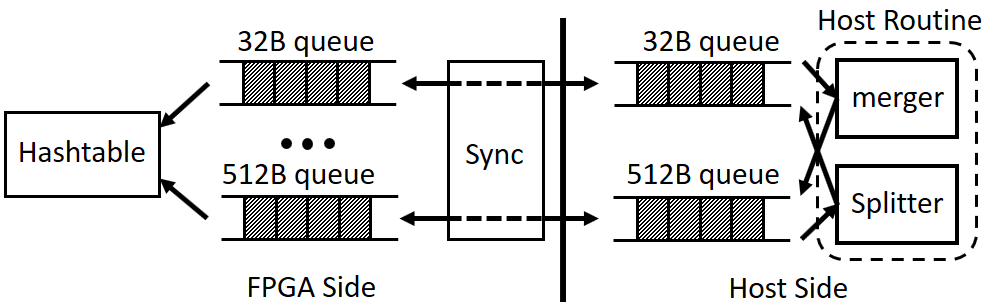
\includegraphics[width=.5\textwidth,page=1]{slab.PNG}
\caption{Slab memory allocator.}
\label{fig:slab}
\vspace{-10pt}
\end{figure}

As shown in Figure~\ref{fig:slab}, for each slab size, the free slab pool is organized as a double-ended queue.
One end of the queue is accessed and cached by the NIC, the other end is accessed by the CPU.
Each slab cache is also a double-ended queue on the NIC, one end popped and pushed by the allocator and deallocator, the other end synced with host memory in batches.
Each double-ended queue has a high watermark and a low watermark.
When the host queue size grows above the high watermark, slab merging is triggered; when it drops below the low watermark, slab splitting is triggered.
The cache on NIC is synchronized with host DRAM in batches according to high and low watermarks.

%\textbf{Dynamic Operation Scheduler.}
%Upon simultaneous completion of an operation and arrival of a new operation, the reservation station prioritizes completion processing, because the completed operation has waited longer and prioritizing it benefits tail latency.
%During checking and execution of a hash slot, new completions may come.
%For simplicity, we finish scanning the chain of pending operations before moving to another key.

\textbf{DRAM Load Dispatcher.}
One technical challenge is the storage of metadata in DRAM cache, which requires additional 4 address bits and one dirty flag per 64-byte cache line.
Cache valid bit is not needed because all KVS storage is accessed exclusively by the NIC.
To store the 5 metadata bits per cache line, extending the cache line to 65 bytes would reduce DRAM performance due to unaligned access; saving the metadata elsewhere will double memory accesses.
Instead, we leverage spare bits in ECC DRAM for metadata storage.
ECC DRAM typically has 8 ECC bits per 64 bits of data.
For Hamming code to correct one bit of error in 64 bits of data, only 7 additional bits are required.
The 8th ECC bit is a parity bit for detecting double-bit errors.
As we access DRAM in 64-byte granularity and alignment, there are 8 parity bits per 64B data.
We increase the parity checking granularity from 64 data bits to 256 data bits, so double-bit errors can still be detected. This allows us to have 6 extra bits which can save our address bits and dirty flag.

%\textbf{KV Operation Decoder.}
%The KV operation decoder saves receive timestamp and UDP flow tuple as execution context in reservation station.
%When the KV operation completes, the flow control component measures the processing delay from the receive timestamp in execution context.
%The network encoder needs the flow tuple to generate completion packets and send to the client.
%To avoid head-of-line blocking, KV operations are processed out-of-order, so the client may receive KV completions in a different order from requests.
%The client could match the completions with requests by the key, because completions with a same key are guaranteed to be in request order.

\textbf{Vector Operation Decoder.}
%Throughout the KV processor design, we see batching as an universal principle in fetching multiple hash slots in one bucket, synchronizing free slab queues with host memory, lazy splitting and merging of slab slots, and data forwarding of dependent KV operations.
%Batching improves performance by amortizing control plane overhead to multiple data plane payloads.
Compared with PCIe, network is a more scarce resource with lower bandwidth (5~GB/s) and higher latency (2~$\mu$s).
%The control plane overhead of network is also larger. 
An RDMA write packet over Ethernet has 88 bytes of header and padding overhead, while a PCIe TLP packet has only 26 bytes of overhead.
This calls for network batching in two aspects: batching multiple KV operations in one packet and supporting vector operations for a more compact representation. Towards this end, we implement a decoder in the KV-engine to unpack multiple KV operations from a single RDMA packet.
%For computation efficiency, we could not use a general-purpose compression algorithm.
%Observing that many KVs have a same size or repetitive values, the KV format includes two flag bits to allow copying key and value size or the value part of the previous KV in the packet.
%For atomic and vector operations, additional fields include the opcode of the $\lambda$ function and the parameter to the active message.
\section{Evaluation}

\begin{figure}[t]
\begin{minipage}[t]{0.5\textwidth}
\subfloat[Fix memory utilization.\label{fig:optimize_fix_mem}]
{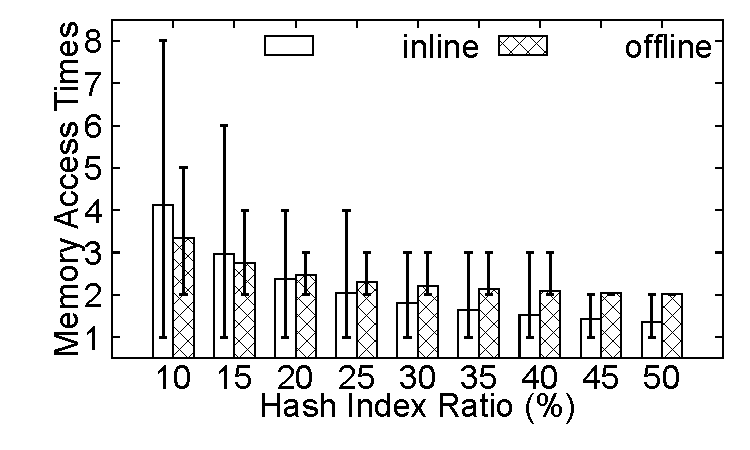
\includegraphics[width=.5\textwidth,page=1]{fix_mem.pdf}}
\subfloat[Fix hash index ratio.\label{fig:optimize_fix_ratio}]
{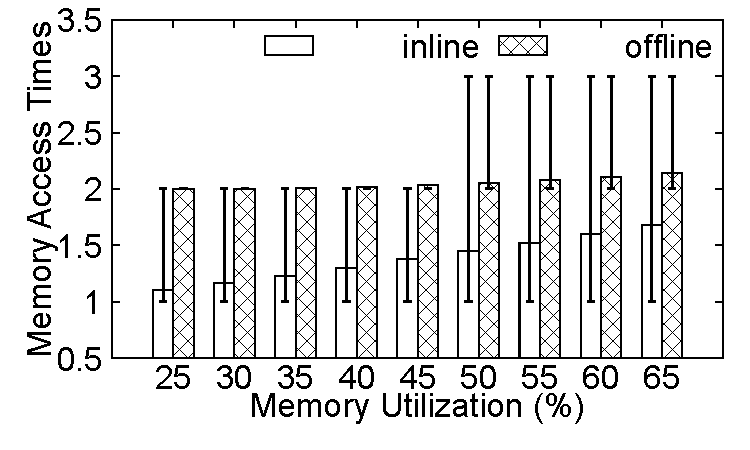
\includegraphics[width=.5\textwidth,page=1]{fix_ratio.pdf}}
\caption{Memory access count under different memory utilizations or hash index ratio.}
\end{minipage}
\vspace{-10pt}
\end{figure}

\begin{figure}[t]
\centering
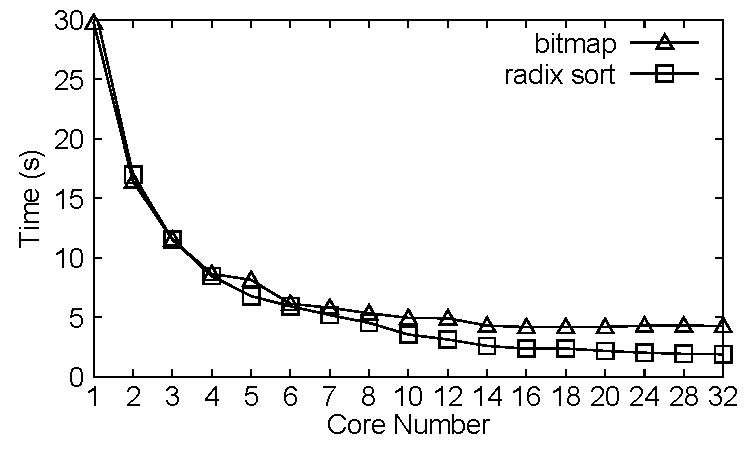
\includegraphics[width=0.33\textwidth]{slab-gc.pdf}
\caption{Execution time of merging 4 billion slab slots.}
\label{fig:slab-garbage-collection}
\vspace{-8pt}
\end{figure}

\begin{figure}[t]
\centering
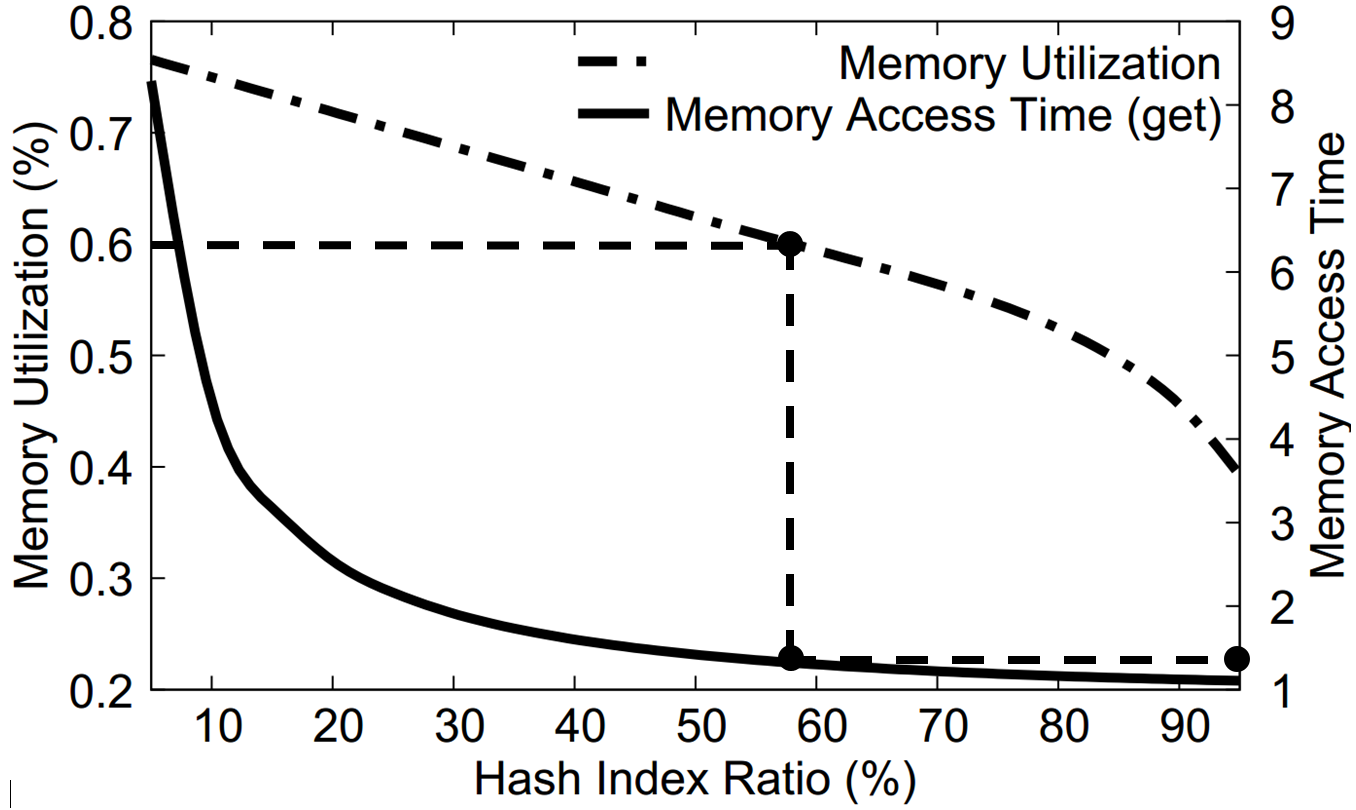
\includegraphics[width=0.33\textwidth,page=1]{optimize.png}
\caption{Determining the optimal hash index ratio for a required memory utilization and KV size.}
\label{fig:hashline-ratio}
\vspace{-8pt}
\end{figure}

\label{sec:evaluation}
In this section, we first take a reductionist perspective to support our design choices with microbenchmarks of key components, then switch to a holistic approach to demonstrate the overall performance of \oursys{} in system benchmark.

\label{sec:evaluation-setup}
We evaluate KV-Direct in a testbed of 32 Dell R730 servers and 10 Arista DCS-7060CX-32S switches in fat-tree topology.
Each server equips two 16 core Xeon E5-2698 v3 CPUs with hyper-threading disabled, forming two NUMA nodes connected through QPI Link. Each NUMA node is populated with 4 DIMMs of 32~GiB DDR4-2400 ECC RAM, resulting a total of 256~GiB of system memory on each server.
A programmable NIC is connected to the PCIe complex of CPU 0, and its 40~Gbps Ethernet port is connected to a Top-of-Rack (ToR) switch.

For system benchmark, we use YCSB workload~\cite{cooper2010benchmarking}.
For skewed Zipf workload, we choose skewness 0.99 and refer it as \textit{long-tail} workload.

\subsection{Microbenchmarks}
\label{sec:microbenchmarks}


\subsubsection{Hash Table}
\label{sec:hashtable-eval}

There are two free parameters in our hash table design: (1) inline threshold, (2) the ratio of hash index in the entire memory space.
As shown in Figure~\ref{fig:optimize_fix_mem}, when hash index ratio grows, more KV pairs can be stored inline, yielding a lower average memory access time.
Figure~\ref{fig:optimize_fix_ratio} shows the increase of memory access time as more memory is utilized.
We use memory utilization instead of load factor, because it relates more to the number of KVs that can fit in a fixed amount of memory.
As shown in Figure~\ref{fig:hashline-ratio}, the maximal achievable memory utilization drops under higher hash index ratio, because less memory is available for dynamic allocation.
Consequently, aiming to accommodate the entire corpus in a given memory size, the hash index ratio has an upper bound.
We choose this upper bound and get a minimal average memory access times, shown as the dashed line in Figure~\ref{fig:hashline-ratio}.

\begin{figure}[t]
\centering
\subfloat[10B GET.\label{fig:mem-access-10-get}]
{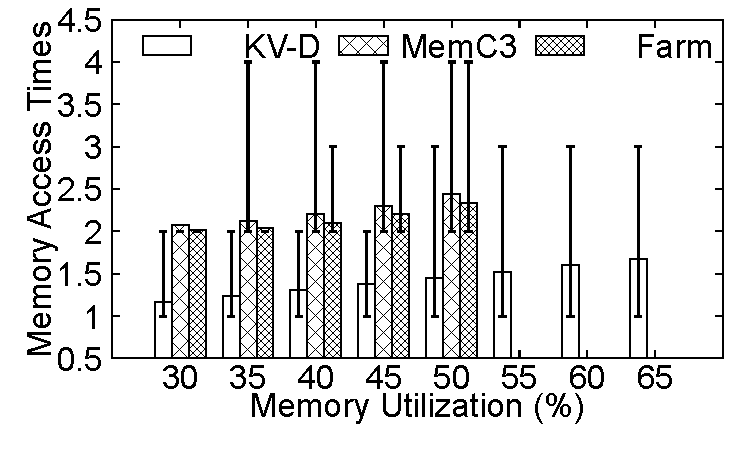
\includegraphics[width=.25\textwidth,page=1]{10B_get.pdf}}
\subfloat[10B PUT.\label{fig:mem-access-10-put}]
{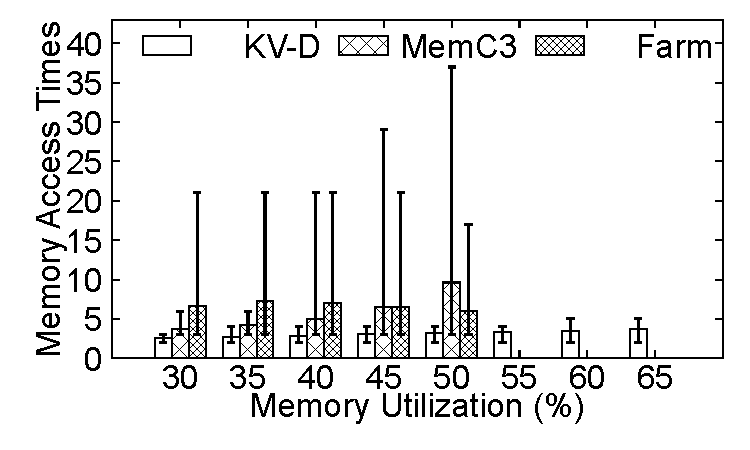
\includegraphics[width=.25\textwidth,page=1]{10B_put.pdf}}

\vfill

\subfloat[254B GET.\label{fig:mem-access-254-get}]
{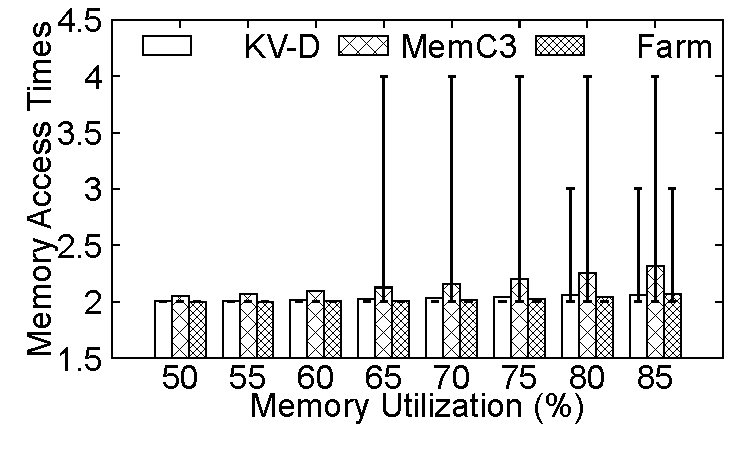
\includegraphics[width=.25\textwidth,page=1]{254B_get.pdf}}
\subfloat[254B PUT.\label{fig:mem-access-254-put}]
{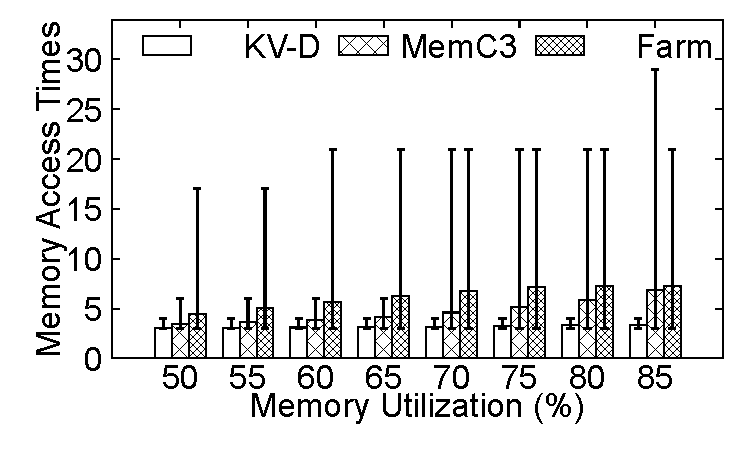
\includegraphics[width=.25\textwidth,page=1]{254B_put.pdf}}
\caption{Memory accesses per KV operation.}
\label{fig:mem-access-tput}
\vspace{-10pt}
\end{figure}

In Figure~\ref{fig:mem-access-tput}, we plot the number of memory accesses per GET and PUT operation for three possible hash table designs: chaining in KV-Direct, bucket cuckoo hashing in MemC3~\cite{fan2013memc3} and chain-associative hopscotch hashing in FaRM~\cite{dragojevic2014farm}.
For KV-Direct, we make the optimal choice of inline threshold and hash index ratio for the given KV size and memory utilization requirement.
For cuckoo and hopscotch hashing, we assume that keys are inlined and can be compared in parallel, while the values are stored offline.
Since the hash table of MemC3 and FaRM cannot support more than 55\% memory utilization for 10B KV size, the three rightmost bars in Figure~\ref{fig:mem-access-10-get} and Figure~\ref{fig:mem-access-10-put} only show the performance of KV-Direct.

For inline KVs, KV-Direct has close to 1 memory access per GET and close to 2 memory accesses per PUT under non-extreme memory utilizations.
GET and PUT for non-inline KVs have one additional memory access.
Comparing KV-Direct and chained hopscotch hashing under high memory utilization, hopscotch hashing performs better in GET, but significantly worse in PUT.
Cuckoo hashing needs to access up to two hash slots on GET, therefore has more memory accesses than KV-Direct under most memory utilizations.
Under high memory utilization, cuckoo hashing incurs large fluctuations in memory access times per PUT.


\subsubsection{Slab Memory Allocator}
\label{sec:slab-eval}

The communication overhead of slab memory allocator comes from the NIC accessing available slab queues in host memory.
To sustain the maximal throughput of 180M operations per second, in the worst case, 180M slab slots need to be transferred, consuming 720 MB/s PCIe throughput, \ie, 5\% of total PCIe throughput of our NIC.

The computation overhead of slab memory allocator comes from slab splitting and merging on host CPU.
Fortunately, they are not frequently invoked.
For workloads with stable KV size distributions, newly freed slab slots are reused by subsequent allocations, therefore does not trigger splitting and merging.

Slab splitting requires moving continuous slab entries from one slab queue to another. When the workload shifts from large KV to small KV, in the worst case the CPU needs to move 90M slab entries per second, which only utilizes 10\% of a core because it is simply continuous memory copy.

Merging free slab slots to larger slots is rather a time-consuming task, because it involves filling the allocation bitmap with potentially random offsets and thus requiring random memory accesses.
To sort the addresses of free slabs and merge continuous ones, radix sort~\cite{satish2010fast} scales better to multiple cores than simple bitmap.
As shown in Figure~\ref{fig:slab-garbage-collection}, merging all 4 billion free slab slots in a 16 GiB vector requires 30 seconds on a single core, or only 1.8 seconds on 32 cores using radix sort~\cite{satish2010fast}.
Although garbage collecting free slab slots takes seconds, it runs in background without stalling the slab allocator, and practically only triggered when the workload shifts from small KV to large KV.

\begin{figure}[t]
\centering
\subfloat[Atomics.\label{fig:ooo-atomic}]
{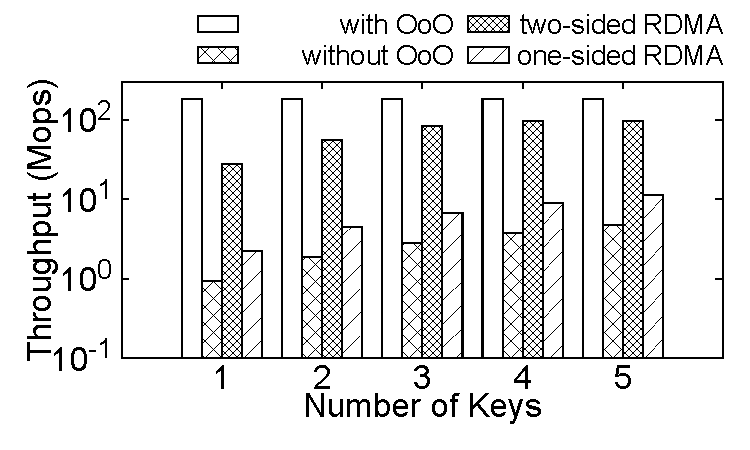
\includegraphics[width=.25\textwidth,page=1]{ooo_atomic.pdf}}
\subfloat[Long-tail workload.\label{fig:ooo-longtail}]
{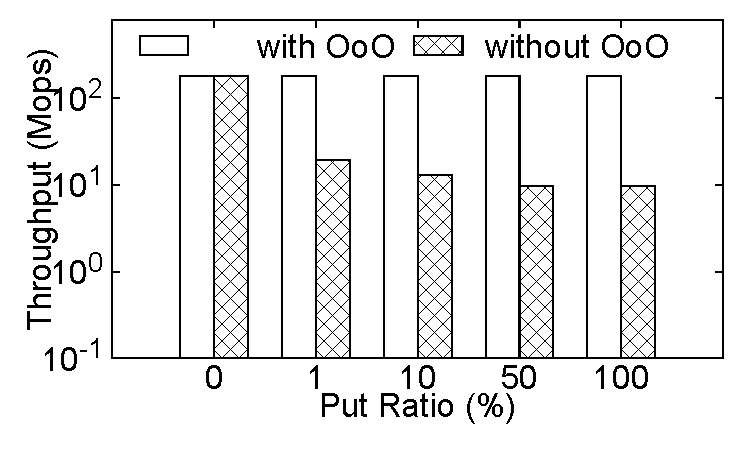
\includegraphics[width=.25\textwidth,page=1]{ooo_long-tail.pdf}}
\caption{Effectiveness of out-of-order execution engine.}
\label{fig:ooo-eval}
\vspace{-20pt}
\end{figure}

\begin{figure}[t]
\centering
{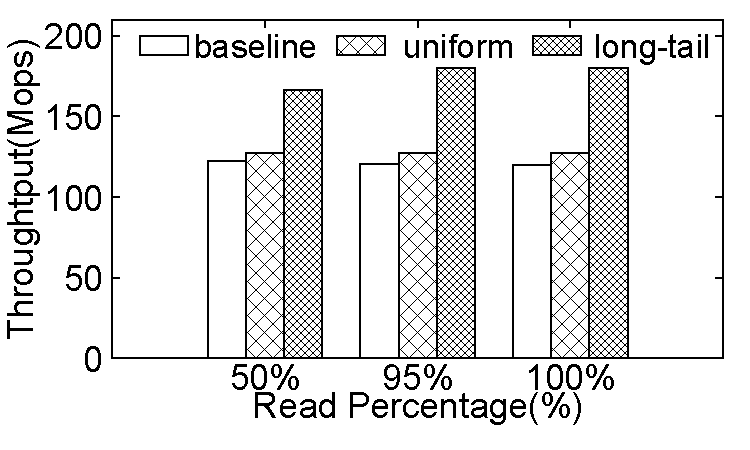
\includegraphics[width=.25\textwidth,page=1]{load_balancer.pdf}}
\caption{DMA throughput with load dispatch. Load dispatch ratio is 0.5.}
\label{fig:cache-tput}
\vspace{-25pt}
\end{figure}

\begin{figure}[t]
\centering
\subfloat[Throughput.\label{fig:network-batching-bw}]
{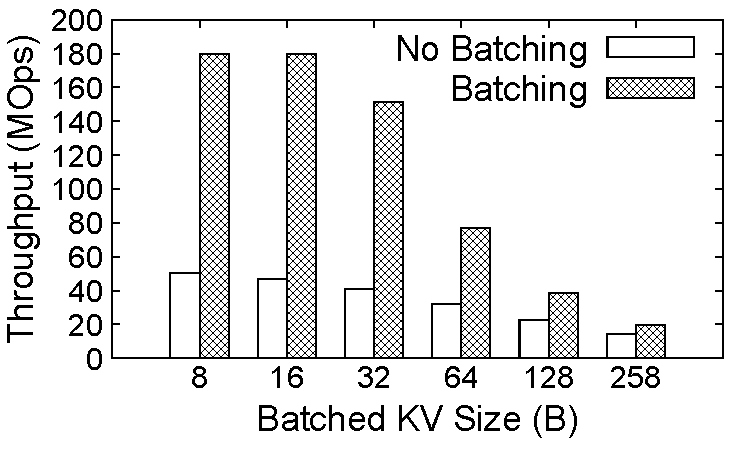
\includegraphics[width=.25\textwidth,page=1]{net_batching_bw.pdf}}
\subfloat[Latency.\label{fig:network-batching-bw}]
{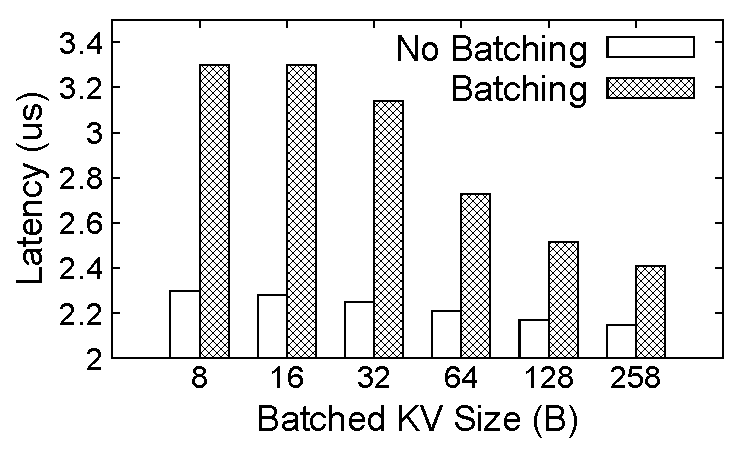
\includegraphics[width=.25\textwidth,page=1]{net_batching_lat.pdf}}
\caption{Efficiency of network batching.}
\label{fig:eval-network-batching}
\vspace{-15pt}
\end{figure}

\subsubsection{Out-of-Order Execution Engine}
\label{sec:ooo-eval}

We evaluate the effectiveness of out-of-order executing by comparing the throughput with one-sided RDMA and two-sided RDMA~\cite{kalia2016design}, under atomics and skewed workload using the simple approach that stalls the pipeline on key conflict.

Without this engine, an atomic operation needs to wait for PCIe latency and processing delay in the NIC, during which subsequent atomic operations on the same key cannot be executed.
This renders a single-key atomics throughput of 0.94~Mops in Figure~\ref{fig:ooo-atomic}, consistent with 2.24~Mops measured from an RDMA NIC~\cite{kalia2016design}.
The higher throughput of RDMA NIC can be attributed to its higher clock frequency and lower processing delay.
With out-of-order execution, single-key atomic operations in KV-Direct can be processed at peak throughput, \ie, one operation per clock cycle.
In MICA~\cite{li2016full}, single-key atomics throughput cannot scale beyond a single core.
Atomic fetch-and-add can be spread to multiple cores in~\cite{kalia2016design}, but it relies on the commutativity among the atomics and therefore does not apply to non-commutative atomics such as compare-and-swap.

With out-of-order execution, single-key atomics throughput improves by 191x and reaches the clock frequency bound of 180~Mops.
When the atomic operations spread uniformly among multiple keys, the throughput of one-sided RDMA, two-sided RDMA and KV-Direct without out-of-order execution grow linearly with the number of keys, but still far from the optimal throughput of KV-Direct.

Figure~\ref{fig:ooo-longtail} shows the throughput under the long-tail workload.
Recall that the pipeline is stalled when a PUT operation finds any in-flight operation with the same key.
The long-tail workload has multiple extremely popular keys, so it is likely that two operations with the same popular key arrive closely in time.
With higher PUT ratio, it is more likely that at least one of the two operations is a PUT, therefore triggering a pipeline stall.


\subsubsection{DRAM Load Dispatcher}
\label{sec:dram-eval}

Figure~\ref{fig:cache-tput} shows the throughput improvement of DRAM load dispatch over the baseline of using PCIe only.
Under uniform workload, the caching effect of DRAM is negligible because its size is only 6\% of host KVS memory.
Under long-tail workload, \approx30\% of memory accesses are served by the DRAM cache. Overall, the memory access throughput for 95\% and 100\% GET achieves the 180 Mops clock frequency bound.
However, if DRAM is simply used as a cache, the throughput would be adversely impacted because the DRAM throughput is lower than PCIe throughput.

\subsubsection{Vector Operation Decoder}
\label{network-eval}

\begin{table}[]
\centering
\scalebox{0.75}{
\begin{tabular}{|l|r|r|r|r|r|}
\hline
Vector Size (B)              & 64    & 128   & 256   & 512   & 1024  \\ \hline
Vector update with return    & 11.52 & 11.52 & 11.52 & 11.52 & 11.52 \\ \hline
Vector update without return & 4.37  & 4.53  & 4.62  & 4.66  & 4.68  \\ \hline
One key per element          & 2.09  & 2.09  & 2.09  & 2.09  & 2.09  \\ \hline
Fetch to client              & 0.03  & 0.06  & 0.12  & 0.24  & 0.46  \\ \hline
\end{tabular}
}
\caption{Throughput (GB/s) of vector operations with vector update or alternatives.}
\label{tab:vec_throughput}
\vspace{-15pt}
\end{table}

To evaluate the efficiency of vector operations in KV-Direct, Table~\ref{tab:vec_throughput} compares the throughput of atomic vector increment with two alternative approaches:
(1) If each element is stored as a unique key, the bottleneck is the network to transfer the KV operations.
(2) If the vector is stored as a large opaque value, retrieving the vector to the client also overwhelms the network.
Additionally, the two alternatives in Table~\ref{tab:vec_throughput} do not ensure consistency within the vector. Adding synchronization would incur further overhead.

KV-Direct client packs KV operations in network packets to mitigate packet header overhead.
Figure~\ref{fig:eval-network-batching} shows that network batching increases network throughput by up to 4x, while keeping networking latency below 3.5 microseconds.

\egg{
\subsubsection{Congestion Avoidance}
\label{congestion-avoidance}

We evaluate the efficiency of congestion avoidance using the KV size distribution of the USR pool in Facebook memcached workload~\cite{atikoglu2012workload}.
As shown in Figure~\ref{fig:congestion-avoidance}, without congestion avoidance, about 70\% KV operations complete with close to one PCIe RTT latency, while remaining 30\% operations have inflated completion times due to explicit and implicit queuing in the KV processor.
With congestion avoidance, the rate for the programmable NIC to accept KV operations from clients is dynamically adjusted, therefore $>$~90\% KV operations complete with close to one PCIe RTT latency.
The remaining few percent of operations have intrinsic higher processing delay due to their larger KV sizes.
}

\subsection{System Benchmark}
\label{sec:system-benchmark}

\subsubsection{Methodology}

Before each benchmark, we tune hash index ratio, inline threshold and load dispatch ratio according to the KV size, access pattern and target memory utilization.
Then we generate random KV pairs and issue PUT operations to insert them into an idle KVS until 50\% memory utilization.
The performance under other memory utilizations can be derived from Figure~\ref{fig:mem-access-tput}.

During benchmark, we use an FPGA-based packet generator~\cite{li2016clicknp} in the same ToR to generate batched KV operations, send them to the KV server, receive completions and measure sustainable throughput and latency.
The processing delay of the packet generator is pre-calibrated via direct loop-back and removed from latency measurements.
Error bars represent the $5^{th}$ and $95^{th}$ percentile.

\subsubsection{Throughput and power efficiency}

\begin{table*}[h]
\centering
\scalebox{0.8}{
\begin{tabular}{|l|l|l|r|r|r|r|r|r|r|}
\toprule
KVS  & Comment & Bottleneck & \multicolumn{2}{c|}{Throughput (Mops)} & \multicolumn{2}{c|}{Power (Kops/W)} & \multicolumn{2}{c|}{Avg Latency (us)} \\
\cline{4-9}
 & & & GET & PUT & GET & PUT & GET & PUT \\
\midrule
Memcached~\cite{fitzpatrick2004distributed} & Traditional & Core synchronization & 1.5 & 1.5 & \approx5 & \approx5 & \approx300 & \approx300 \\
MemC3~\cite{fan2013memc3} & Traditional & OS network stack & 4.3 & 4.3 & \approx14 & \approx14 & \approx300 & \approx300 \\
RAMCloud~\cite{ousterhout2015ramcloud} & Kernel bypass & Dispatch thread & 6 & 1 & \approx20 & \approx3.3 & 5 & 14 \\
MICA'16~\cite{li2016full} & Kernel bypass, 24 cores, 12 NIC ports & CPU KV processing & 137 & 135 & 342 & 337 & 81 & 81 \\
FaRM~\cite{dragojevic2014farm} & One-sided RDMA for GET & RDMA NIC & 6 & 3 & \approx600 & \approx20 & 4.5 & \approx10 \\
DrTM-KV~\cite{wei2015fast} & One-sided RDMA and HTM & RDMA NIC & 115.2 & 14.3 & \approx400 & \approx50 & 3.4 & 6.3 \\
HERD'16~\cite{kalia2016design} & Two-sided RDMA, 12 cores & PCIe & 98.3 & \approx60 & \approx300 & \approx200 & 5 & 5 \\
Xilinx'13~\cite{blott13hotcloud} & FPGA (with host) & Network & 13 & 13 & 106 & 106 & 3.5 & 4.5 \\
Mega-KV~\cite{zhang2015mega} & GPU (4~GiB on-board RAM) & GPU KV processing & 166 & 80 & \approx330 & \approx160 & 280 & 280 \\
\midrule
\textbf{KV-Direct (1 NIC)} & Programmable NIC, two Gen3x8 hardIPs & PCIe \& DRAM & 180 & 114 & 6600 & 4200 & 4.3 & 5.4 \\
\textbf{KV-Direct (8 NICs)} & Programmable NIC, one Gen3x8 hardIP each & PCIe \& DRAM & 1020 & 508 & 2732 & 1385 & 4.3 & 5.4 \\
\bottomrule
\end{tabular}
}
\caption{Comparison of KV-Direct with other KVS systems under long-tail (skewed Zipf) workload of 10B tiny KVs. For metrics not reported in the papers, we emulate the systems using similar hardware and report our approximate measurements.}
\label{tab:kvs-compare}
\vspace{-15pt}
\end{table*}

\begin{figure}[t]
\centering
\subfloat[Uniform.\label{fig:ycsb-tput-uniform}]
{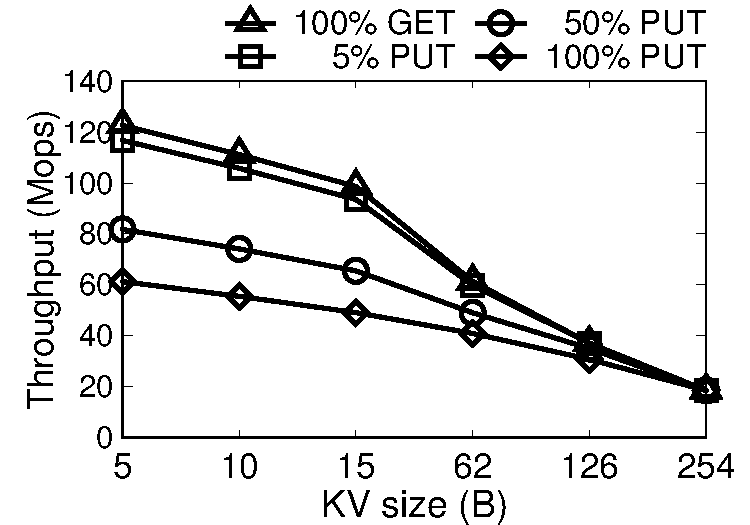
\includegraphics[width=.25\textwidth,page=1]{ycsb-tput-uniform.pdf}}
\subfloat[Long-tail.\label{fig:ycsb-tput-longtail}]
{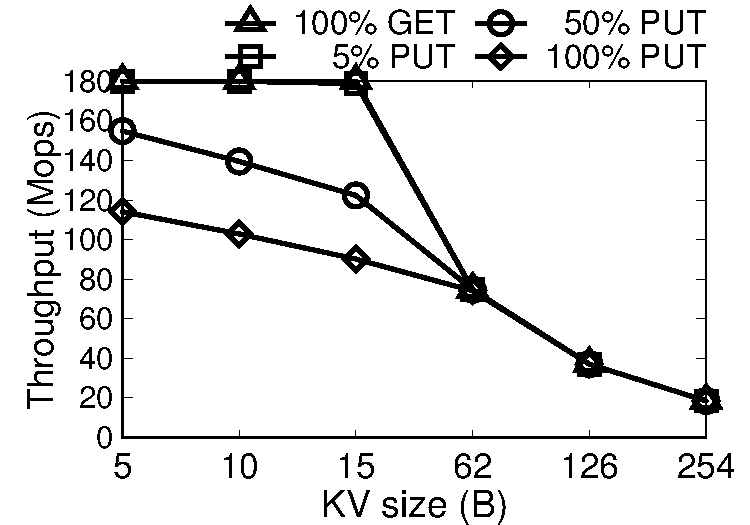
\includegraphics[width=.25\textwidth,page=1]{ycsb-tput-longtail.pdf}}
\caption{Throughput of KV-Direct under YCSB workload.}
\label{fig:ycsb-tput}
\vspace{-10pt}
\end{figure}

Figure~\ref{fig:ycsb-tput} shows the throughput of KV-Direct under YCSB uniform and long-tail (skewed Zipf) workload.
Three factors may be the bottleneck of KV-Direct: clock frequency, network and PCIe/DRAM.
For 5B\approx15B KVs inlined in the hash index, most GETs require one PCIe/DRAM access and PUTs require two PCIe/DRAM accesses.
Under same memory utilization, larger inline KVs have lower throughput, due to a higher probability of hash collision.
62B and larger KVs are not inlined, so they require an additional memory access.
Long-tail workload has higher throughput than uniform workload and able to reach the clock frequency bound of 180~Mops under read-intensive workload, or reach the network throughput bound for $\geq$62B KV sizes.
Under long-tail workload, the out-of-order execution engine merges up to \approx15\% operations on the most popular keys, and the on-board DRAM has \approx60\% cache hit rate under 60\% load dispatch ratio, which collectively leads to up to 2x throughput as uniform workload.
As shown in Table~\ref{tab:kvs-compare}, the throughput of a KV-Direct NIC is on-par with a state-of-the-art KVS server with tens of CPU cores.

%When the KV-Direct NIC is unplugged, an idle server consumes 207W wall power on average.
%By plugging the KV-Direct NIC onto the server and connecting the NIC to the network, the server consumes 10W additional power.
%When the KV-Direct NIC is at peak throughput under long-tail workload, the server consumes 234W average wall power.
%So we conclude that the peak power utilization of KV-Direct is 27W.
We measure the power difference of a KV-Direct server at peak throughput and at idle to be 27 watts, which is the combined power consumption of reconfigurable NIC, PCIe, host memory and the daemon process on CPU.
Compared with state-of-the-art KVS systems in Table~\ref{tab:kvs-compare}, KV-Direct is 10\approx20x more power efficient than CPU-based systems, as well as being the first general-purpose in-host-memory KVS system to achieve $>$~1M KV operations per watt. Measuring the power difference is justified since the CPU is almost idle and the server can run other workloads when KV-Direct is operating (we use the same criterion for GET operation of FaRM in Table~\ref{tab:kvs-compare}).
If the server base idle power (207W) is not deducted, the power efficiency for PUT and GET will be reduced to 769 Kops/W and 487 Kops/W respectively, still much better than other KVS systems.
\subsubsection{Latency}
\begin{figure}[t]
\centering
\subfloat[With batching.\label{fig:ycsb-lat-batch}]
{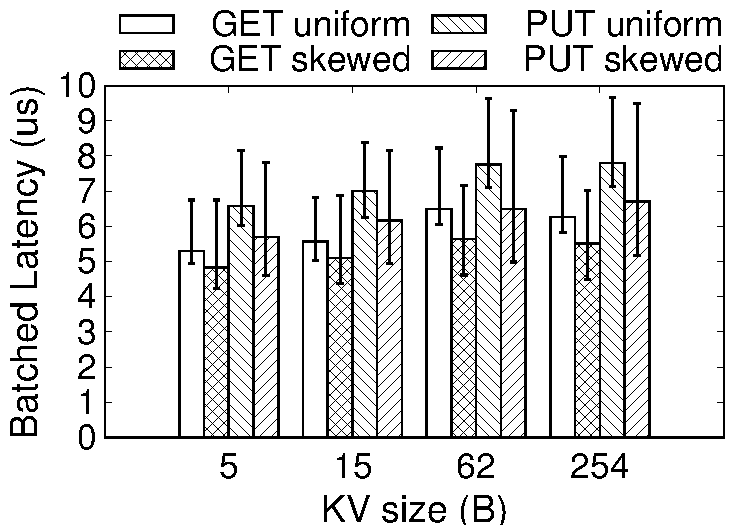
\includegraphics[width=.25\textwidth,page=1]{lat-batch.pdf}}
\subfloat[Without batching.\label{fig:ycsb-lat-nobatch}]
{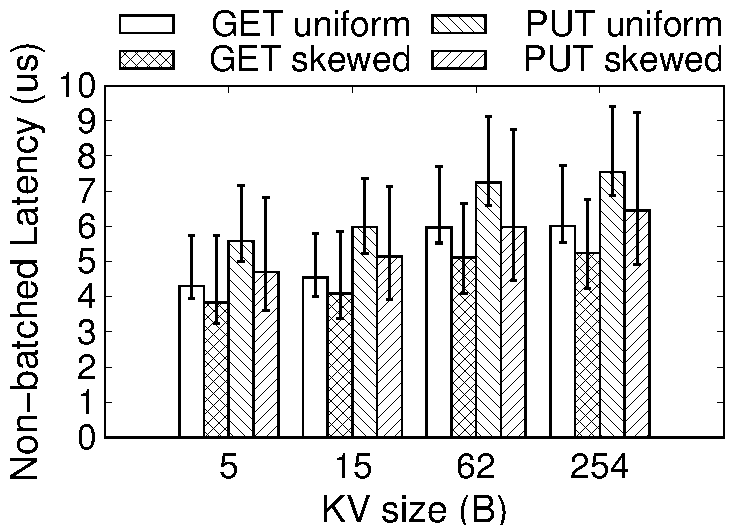
\includegraphics[width=.25\textwidth,page=1]{lat-nonbatch.pdf}}
\caption{Latency of KV-Direct under peak throughput of YCSB workload.}
\label{fig:ycsb-lat}
\vspace{-15pt}
\end{figure}

Figure~\ref{fig:ycsb-lat} shows the latency of KV-Direct under the peak throughput of YCSB workload.
Without network batching, the tail latency ranges from 3\approx9~$\mu$s depending on KV size, operation type and key distribution.
PUT has higher latency than GET due to additional memory access.
Skewed workload has lower latency than uniform due to more likelihood of being cached in on-board DRAM.
Larger KV has higher latency due to additional network and PCIe transmission delay.
Network batching adds $< 1 \mu$s latency than non-batched operations, but significantly improves throughput, which has been evaluated in Figure~\ref{fig:eval-network-batching}.

\subsubsection{Impact on CPU performance}

\begin{table}[t!]
	\centering
	\scalebox{0.8}{
		\begin{tabular}{l|l|r|r}
			\toprule
			\multicolumn{2}{r}{KV-Direct status $\rightarrow$} & Idle & Busy \\
			\midrule
			\multirow{4}{*}{\specialcell{Random\\Latency}} & CPU0-0 & 82.2 ns & 83.5 ns \\
            					  & CPU0-1 & 129.3 ns & 129.9 ns \\
                                  & CPU1-0 & 122.3 ns & 122.2 ns \\
                                  & CPU1-1 & 84.2 ns & 84.3 ns \\
			\midrule
            \multirow{4}{*}{\specialcell{Sequential\\Throughput}} & \textbf{CPU0-0} & \textbf{60.3 GB/s} & \textbf{55.8 GB/s} \\
            					  & CPU0-1 & 25.7 GB/s & 25.6 GB/s \\
                                  & CPU1-0 & 25.5 GB/s & 25.9 GB/s \\
                                  & CPU1-1 & 60.2 GB/s & 60.3 GB/s \\
			\midrule
			\multirow{4}{*}{\specialcell{Random\\Throughput}} & 32B read & 10.53 GB/s & 10.46 GB/s \\
            						& 64B read & 14.41 GB/s & 14.42 GB/s \\
                                    & 32B write & 9.01 GB/s & 9.04 GB/s \\
                                    & 64B write & 12.96 GB/s & 12.94 GB/s \\
			\bottomrule
		\end{tabular}
	}
    	\caption{Impact on CPU memory access performance when KV-Direct is at peak throughput.}
        \label{tab:cpu-impact}
        \vspace{-5pt}
\end{table}


KV-Direct is designed to bypass the server CPU and uses only a portion of host memory for KV storage. Therefore, the CPU can still run other applications.
Our measurements find a minimal impact on other workloads on the server when a single NIC KV-Direct is at peak load.
Table~\ref{tab:cpu-impact} quantifies this impact at the peak throughput of KV-Direct.
Except for sequential throughput of CPU 0 to access its own NUMA memory (the line marked in bold), the latency and throughput of CPU memory accesses are mostly unaffected.
This is because 8 channels of host memory can provide far higher random access throughput than all CPU cores could consume, while the CPU can indeed stress the sequential throughput of the DRAM channels.
The impact of the host daemon process is minimal when the distribution of KV sizes is relatively stable, because the garbage collector is invoked only when the number of available slots for different slab sizes are imbalanced (\S\ref{sec:slab}).

\section{Extensions}
\label{sec:extensions}

\subsection{CPU-based Scatter-Gather DMA}

PCIe has 29\% TLP header and padding overhead for 64B DMA operations (\S\ref{sec:challenge}) and the DMA engine may not have enough parallelism to saturate the PCIe bandwidth-delay product with small TLPs (\S\ref{sec:implementation}).
Larger DMA operations with up to 256-byte TLP payload is supported by the PCIe root complex in our system. In this case, the TLP head and padding overhead is only 9\%, and the DMA engine has enough parallelism (64) to saturate the PCIe link with 27 in-flight DMA reads.
To batch the DMA operations on PCIe link, we can leverage the CPU to perform scatter-gather (Figure~\ref{fig:sg-arch}).
First, the NIC DMAs addresses to a request queue in host memory. The host CPU polls the request queue, performs random memory access, put the data in response queue and writes MMIO doorbell to the NIC. The NIC then fetches the data from response queue via DMA.

\begin{figure}[t]
\centering
\subfloat[Read.\label{fig:sge-read}]
{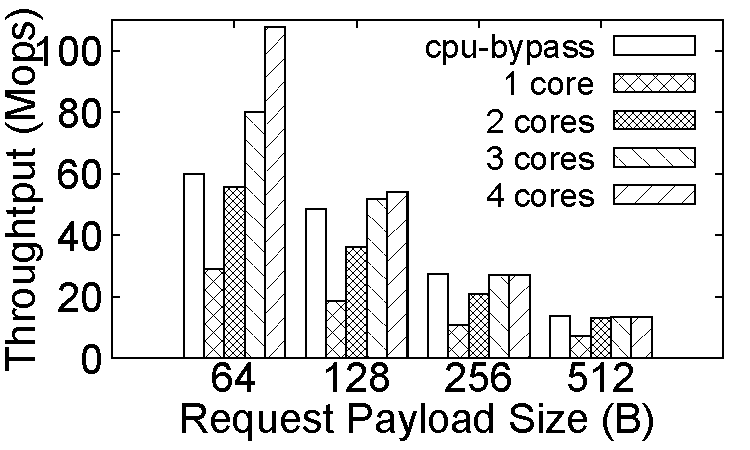
\includegraphics[width=.25\textwidth,page=1]{sg-read.pdf}}
\subfloat[Write.\label{fig:sge-write}]
{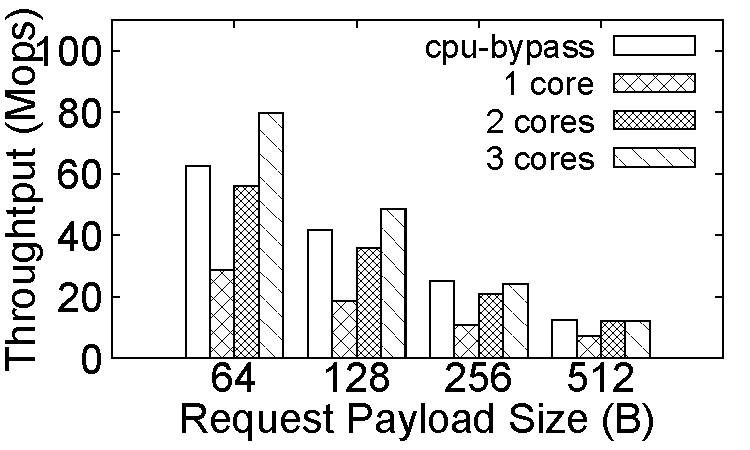
\includegraphics[width=.25\textwidth,page=1]{sg-write.pdf}}
\caption{Scatter-gather performance.}
\label{fig:scatter-gather}
\vspace{-15pt}
\end{figure}

Figure~\ref{fig:scatter-gather} shows that CPU-based scatter-gather DMA has up to 79\% throughput improvement compared to the CPU-bypassing approach.
In addition to the CPU overhead, the primary drawback of CPU-based scatter-gather is the additional latency.
To save MMIOs from the CPU to the NIC, we batch 256 DMA operations per doorbell, which requires 10~$\mu$s to complete.
The overall latency for the NIC to access host memory using CPU-based scatter-gather is \approx20~$\mu$s, almost 20x higher than direct DMA.

\subsection{Multiple NICs per Server}

\begin{figure}[t]
\begin{minipage}[t]{0.23\textwidth}
\centering
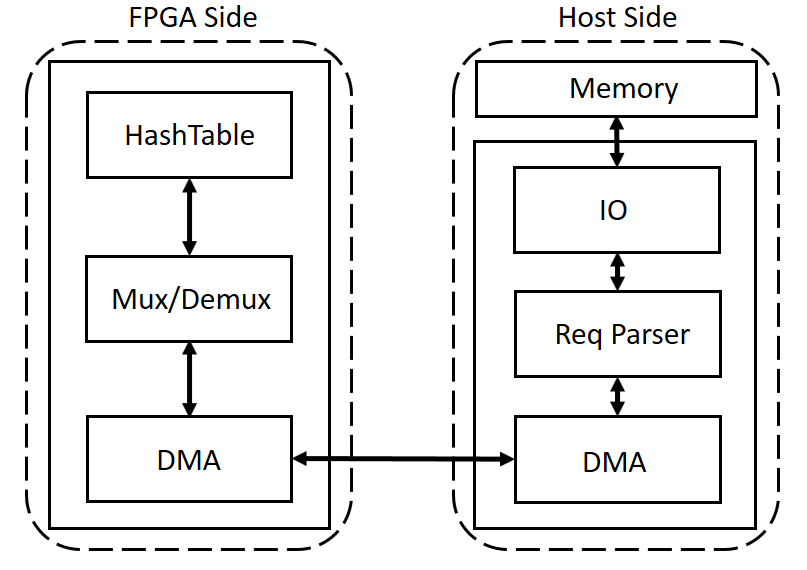
\includegraphics[width=1\textwidth,page=1]{scatter_gather.PNG}
\caption{Scatter-gather architecture.}
\label{fig:sg-arch}
\end{minipage}
\begin{minipage}[t]{0.23\textwidth}
\centering
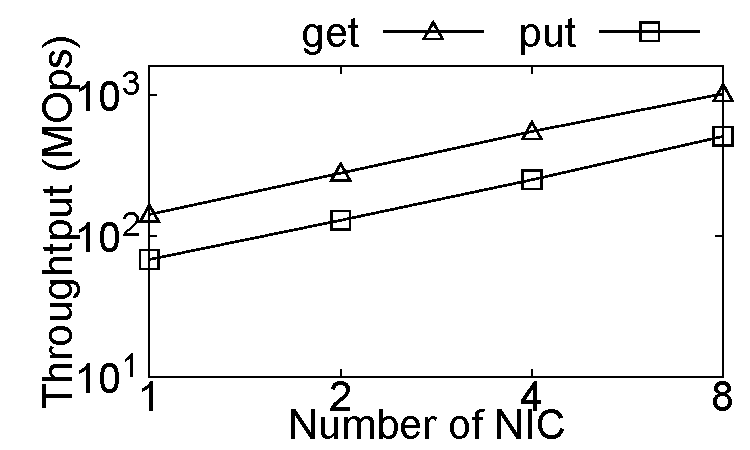
\includegraphics[width=1\textwidth,page=1]{multi_nic.pdf}
\caption{Performance of multiple NICs per server.}
\label{fig:multiple-nics}
\end{minipage}
\vspace{-10pt}
\end{figure}

%The primary use case for KV-Direct is to enable remote direct key-value access without CPU overhead on the server. 
In some cases, it may be desirable to build a dedicated key-value store with maximal throughput per server.
Through simulation, MICA~\cite{li2016full} showed the possibility of achieving a billion KV op/s in a single server with four (currently unavailable) 60-core CPUs.
As shown in Table~\ref{tab:kvs-compare}, with 8 KV-Direct NICs on a server, the one billion KV op/s performance is readily achievable with a commodity server and less than 400 watts of wall power.
The power efficiency for 8 NICs, however, is lower than single NIC, because we accounted for the power of host server.

Due to limited number of full-height PCIe slots in Dell R730 server, for multiple-NIC evaluation, we use an HPE Apollo 6500 server with 8 PCIe Gen3 x16 slots connected to two NUMA CPU nodes via 4 PLX PCIe switches.
Because the HPE server does not support PCIe bifurcation, only one PCIe Gen3 x8 is enabled on each NIC, so the throughput per NIC is lower than Figure~\ref{fig:ycsb-tput}.
Each NIC owns an exclusive memory region in host memory and serves a disjoint partition of keys.
Multiple NICs suffer the same load imbalance problem as a multi-core KVS implementation.
Fortunately, for a small number of partitions (e.g. 8), the load imbalance is not significant~\cite{li2016full}. Under YCSB long-tail workload, the highest-loaded NIC has 1.4x load of the average.
%In comparison, to achieve matching performance with 240 CPU cores, the load of the hottest core will be 10x of the average.
Figure~\ref{fig:multiple-nics} shows that KV-Direct throughput scales linearly with the number of NICs.

\section{Related Work}
\label{sec:related}

As an important infrastructure, the research and development of distributed key-value store systems have been driven by performance. A large body of distributed KVS are based on CPU. To reduce the computation cost, Masstree~\cite{mao2012cache}, MemC3~\cite{fan2013memc3} and libcuckoo~\cite{li2014algorithmic} optimize locking, caching, hashing and memory allocation algorithms, while \oursys{} comes with a new hash table and memory management mechanism specially designed for FPGA to minimize the PCIe traffic. MICA~\cite{lim2014mica, li2016full} partitions the hash table to each core thus completely avoids synchronization. This approach, however, introduces core imbalance for skewed workloads.

To get rid of the OS kernel  overhead, ~\cite{rizzo2012netmap, intel2014data} directly poll network packets from NIC and \cite{, jeong2014mtcp, marinos2014network} process them with the user space lightweight network stack.
Key-value store systems~\cite{kapoor2012chronos, ousterhout2010case, ousterhout2015ramcloud, lim2014mica,li2016full} benefit from such optimizations for high performance.
As a further step towards this direction, recent works \cite{infiniband2000infiniband, kalia2014using, kalia2016design} leverage the hardware-based network stack of RDMA NIC, using two-sided RDMA as an RPC mechanism between KVS client and server to further improve per-core throughput and reduce latency. Still, these systems are CPU bound~\ref{sec:state-of-the-art-kvs}.

Another different approach is to leverage one-sided RDMA. Pilaf~\cite{mitchell2013using}, FaRM~\cite{dragojevic2014farm}, and HERD~\cite{kalia2014using,kalia2016design} adopt one-sided RDMA read for GET operation and achieve NIC-bounded throughput. Nessie~\cite{szepesi2014designing}, DrTM~\cite{wei2015fast}, DrTM+R~\cite{chen2016fast} and FaSST~\cite{kalia2016fasst} leverage distributed transactions to implement both GET and PUT with one-sided RDMA. However, the performance of PUT operation suffer from unavoidable synchronization overhead for consistency guarantee, limited by RDMA primitives~\cite{kalia2016design}. Moreover, client-side CPU is involved in KV processing, limiting per-core throughput to \approx10~Mops on the client side.
In contrast, \oursys{} extends the RDMA primitives to key-value operations while guarantees the consistency in server side, leaving the KVS client totally transparent while achieving high throughput and low latency even for PUT operation.

As a flexible and customizable hardware, FPGA is now widely deployed in datacenter-scale~\cite{putnam2014reconfigurable, caulfield2016cloud} and greatly improved for programmability~\cite{bacon2013fpga,li2016clicknp}. Several early works have explored building KVS on FPGA. But some of them are not practical by limiting the data storage in on-chip (about several MB memory)~\cite{liang16fpl} or on-board DRAM (typically 8GB memory)~\cite{istvan2013flexible,chalamalasetti2013fpga,istvan2015hash}.
~\cite{blott2015scaling} focuses on improving system capacity rather than throughput on FPGA and adopts SSD as the secondary storage out of on-board DRAM.
~\cite{liang16fpl, chalamalasetti2013fpga} limit their usage in fixed size key-value pairs, which can only work for the special purpose rather than a general key-value store.
\cite{blott13hotcloud, lavasani2014fpga} allow the usages of host DRAM by directly applying naive hash table design to FPGA, without considering optimizations for network and PCIe DMA request, resulting in poor performance.
\oursys{} fully utilizes both the on-board DRAM and host DRAM, making our FPGA-based key-value store system general and capable of web-scale production. Furthermore, our careful hardware and software co-design, together with optimizations for PCIe and networking push the performance to the physical limitation, advancing state-of-art solutions.

Secondary index is an important feature to retrieve data by keys other
than the primary key in data storage system~\cite{escriva2012hyperdex, kejriwal2016slik}. SLIK~\cite{kejriwal2016slik} supports multiple secondary keys using a B+ tree algorithm in key-value store system. It would be interesting to explore how to support secondary index to help \oursys{} step towards a general data storage system. SwitchKV~\cite{li2016fast} leverages content-based routing in SDN switches to route requests directly to the cache or backend nodes based on cached keys. Such routing-based load balancing will also benefit our system.

%\textbf{TODO}

%SSD or HDD for persistence~\cite{marmol2014nvmkv, debnath2010flashstore, papagiannis2016tucana}
%network switch~\cite{li2016fast}


%main limitations:

%~\cite{liang16fpl} only uses on-chip BRAM.
%~\cite{istvan2013flexible,chalamalasetti2013fpga,istvan2015hash} only use on-board DRAM, These work don't make use of host RAM, result in small system capacity.

%~\cite{lavasani2014fpga, blott13hotcloud} leverages host RAM, however they didn't have optimization for PCIe DMA which becomes the bottleneck.

%~\cite{liang16fpl, lavasani2014fpga} only support fixed-size Key-value pair, not pratical.


%all works lack of optimization for network like batching and only achieves low encoding efficiency, resulting in low network bandwidth utilization.
%all works lack of optimization for hashtable, which leads to higher average search in heavy load.

\section{Conclusion}
\label{sec:conclusion}
In this paper, we describe the design and evaluation of \oursys{}, a high performance in-memory key-value store. Following a long history in computer system design, \oursys{} is another exercise in leveraging reconfigurable hardware to accelerate an important workload. \oursys{} is able to obtain superior performance by carefully co-designing hardware and software in order to remove bottlenecks in the system and achieve performance that is close to the physical limits of the underlying hardware.

After years of broken promises, FPGA-based reconfigurable hardware  finally becomes widely available in main stream data centers. Many significant workloads will be scrutinized to see whether they can benefit from reconfigurable hardware, and we expect much more fruitful work in this general direction. 

\balance
\bibliographystyle{abbrvnat}
\bibliography{reference}

\end{document}
